\subsection{Construction of continuous sections of étale maps}

THEOREM 1. --- Let X, Y, Z be topological spaces, let \(f: \mathrm{Z} \to \mathrm{X} \times \mathrm{Y}\) be a separated étale morphism, and let \(y_0\) be a point of Y. Let \(s: X \times Y \to Z\) be a section of \(f\) . Assume that the restriction of \(s\) to \(X \times \{y_0\}\) is continuous, as are the restrictions of \(s\) to \(\{x\} \times Y\) for all \(x \in X\). If the space \(Y\) is connected and locally connected (TG, I, p.~84, def. 4), the map \(s\) is continuous.

Lemma. --- Let U be an open subset of X, let V be a connected open subset of Y, and let \((x_{1},y_{1})\in\mathrm{U}\times\mathrm{V}\). Assume that the restriction of s to \(U\times\{y_{1}\}\) is continuous. Let \(\sigma\) be a continuous section of f over \(U\times V\) such that \(\sigma(x_{1},y_{1})=s(x_{1},y_{1})\) . There exists a neighborhood \(U'\) of \(x_{1}\) such that \(s=\sigma\) on \(U'\times V\). In particular, the map s is continuous in a neighborhood of \((x_{1},y_{1})\) .

Since the restriction of \(s\) to \(\mathrm{U} \times \{y_1\}\) is continuous and the map \(f\) is étale, there exists a neighborhood \(\mathrm{U}'\) of \(x_1\) such that \(s(x, y_1) = \sigma(x, y_1)\) for all \(x \in \mathrm{U}'\) (I, p.~34, prop. 11, b)). Let \(x \in \mathrm{U}'\) ; since the restriction of \(s\) to \(\{x\} \times \mathrm{V}\) is continuous and the map \(f\) is étale and separated, it follows from cor. 1, I, p.~34 that \(\sigma(x, y) = s(x, y)\) for all \(y \in \mathrm{V}\) . Thus, \(s\) and \(\sigma\) coincide on \(\mathrm{U}' \times \mathrm{V}\) .

Let us now prove the theorem. Let us first prove that the map s is continuous in a neighborhood of every point of \(X \times \{y_{0}\}\) . Let \(x_{0} \in X\) ; one can choose an open neighborhood U of \(x_{0}\) in X, a connected open neighborhood V of \(y_{0}\) in Y and a continuous section \(\sigma: U \times V \to Z\) of f such that \(\sigma(x_{0}, y_{0}) = s(x_{0}, y_{0})\) . By the lemma above, s is continuous in a neighborhood of \((x_{0}, y_{0})\) .

We now prove that the map \(s\) is continuous at every point of \(\mathrm{X} \times \mathrm{Y}\) . For \(x_0 \in \mathrm{X}\) , denote by \(\mathrm{C}(x_0)\) the set of points \(y \in \mathrm{Y}\) such that \(s\) is continuous in a neighborhood of \((x_0, y)\) . The set \(\mathrm{C}(x_0)\) is open in Y by definition, and contains \(y_0\) by the preceding.

Let us prove that it is closed in Y. Consider a point \(y_{1}\) of Y adherent to \(\mathrm{C}(x_{0})\) , an open neighborhood U of \(x_{0}\) in X, an open neighborhood V of \(y_{1}\) in Y, and a continuous section \(\sigma\colon U\times V\to Z\) of f such that \(\sigma(x_{0},y_{1})=s(x_{0},y_{1})\) . Since the restriction of s to \(\{x_{0}\}\times V\) is continuous and f is étale, there exists an open neighborhood \(V^{\prime}\) of \(y_{1}\) in Y such that \(\sigma(x_{0},y)=s(x_{0},y)\) for all \(y\in V^{\prime}\) (prop. 11 of I, p.~34). Since Y is locally connected, we may assume that \(V^{\prime}\) is connected. Since \(y_{1}\) is adherent to \(\mathrm{C}(x_{0})\), the set \(\mathrm{C}(x_{0})\cap\mathrm{V}^{\prime}\) is nonempty; let \(y_{2}\) be a point of \(\mathrm{C}(x_{0})\cap\mathrm{V}^{\prime}\) . By the lemma applied to \((x_{0},y_{2})\) , there exists a neighborhood \(U^{\prime}\) of \(x_{0}\) contained in U such that \(s=\sigma\) over \(U^{\prime} \times V^{\prime}\) . This proves that \(\mathrm{C}(x_{0})\) is closed, because \(U^{\prime} \times V^{\prime}\) is a neighbourhood of \((x_{0}, y_{1})\) . Since Y is connected, we have \(\mathrm{C}(x_{0}) = \mathrm{Y}\) , and this for every \(x_{0} \in X\) , whence the theorem.

COROLLARY 1. --- Let X, Y, E, B be topological spaces. Let \(p\colon E \to B\) be an étale and separated map, and let \(h\colon X \times Y \to B\) be a continuous map and let \(y_0\) be a point of Y. Let \(g\colon X \times Y \to E\) be a map such that \(p \circ g = h\) . Suppose that the restrictions of \(g\) to \(X \times \{y_0\}\) on the one hand and, for every \(x \in X\) , to \(\{x\} \times Y\) on the other hand, are continuous. If the space Y is connected and locally connected, the map \(g\) is continuous.

Let Z be the fibered product \((\mathrm{X} \times \mathrm{Y}) \times_{\mathrm{B}} \mathrm{E}\) and \(f: Z \to X \times Y\) and \(h': Z \to E\) be the canonical projections. The map f is étale (I, p.~31, prop. 8) and separated (I, p.~27, prop. 4). The map \(s: X \times Y \to Z\) defined by \(s(x, y) = ((x, y), g(x, y))\) is a section of f which satisfies the hypotheses of Theorem 1. It is therefore continuous, as is \(g = h' \circ s\) .

Remark. --- If, in Theorem 1, one does not assume that the space Y is locally connected, the conclusion of the theorem is no longer necessarily valid (I, p.~141, exerc. 7).

THEOREM 2. --- Let B be a topological space and A a subspace of B. Assume one of the following hypotheses:

\begin{enumerate}
\def\labelenumi{(\roman{enumi})}
\item
  A has a fundamental system of paracompact neighborhoods;
\item
  B is paracompact and A is closed;
\item
  B is metrizable;
\item
  A is compact and any two distinct points of A have disjoint neighborhoods in B.
\end{enumerate}

Then, every continuous section over A of an étale map \(p\colon E \to B\) extends to a continuous section of \(p\) over a neighborhood of A.

Consider the following property (PCV) of the pair (B, A):

(PCV) For every covering \((\mathrm{U}_{i})_{i\in\mathrm{I}}\) of A by open subsets of B, there exists a neighborhood V of A and a locally finite family \((\mathrm{F}_{j})_{j\in\mathrm{J}}\) of closed subsets of V covering V, such that each of the \(F_{j}\) is contained in one of the \(U_{i}\) .

Theorem 2 follows from Lemmas 1 and 3 below.

Lemma 1. --- Each of the properties (i) to (iv) of Theorem 2 implies property (PCV).

Let \((\mathrm{U}_{i})_{i\in\mathrm{I}}\) be a covering of A by open subsets of B. Under hypothesis (i), there exists a paracompact neighborhood V of A contained in the union of the \(U_{i}\) , an open covering \((\mathrm{U}_{j}^{\prime})_{j\in\mathrm{J}}\) of the space V, locally finite and finer than the covering \((\mathrm{V}\cap\mathrm{U}_{i})_{i\in\mathrm{I}}\) , and an open covering \((\mathrm{U}_{j}^{\prime\prime})_{j\in\mathrm{J}}\) of the space V such that for every \(j\in J\) , the closure \(F_{j}\) of \(U_{j}^{\prime\prime}\) in V is contained in \(U_{j}^{\prime}\) (TG, IX, p.~49, prop. 4 and p.~48, cor. 1 to th. 3). Hence (PCV) in this case.

Condition (ii) implies condition (i) by Corollary 2 of TG, IX, p.~50. Likewise, condition (iii) implies condition (i): indeed, if B is metrizable, every neighborhood of A is metrizable, hence paracompact (TG, IX, p.~51, th. 4).

Finally suppose condition (iv) is satisfied and let us show that property (PCV) holds. Since A is compact, it suffices to consider the case of a finite covering \((\mathrm{U}_{i})_{0\leqslant i\leqslant n}\) . Let us then construct by induction open sets \(V_{0},\ldots,V_{n}\) of B satisfying the following conditions for \(0\leqslant i\leqslant n\) :

\(\alpha)\mathrm{A}\subset \mathrm{V}_{0}\cup \dots \cup \mathrm{V}_{i}\cup \mathrm{U}_{i + 1}\cup \dots \cup \mathrm{U}_{n};\)

\(\beta)\overline{\mathrm{V}_{i}}\cap \mathrm{A}\subset \mathrm{U}_{i}.\)

Suppose \(V_{0},\ldots,V_{r-1}\) have been constructed satisfying the above conditions for \(0\leqslant i\leqslant r-1\) , and let us construct \(V_{r}\) . The sets \(K=A\cap C U_{r}\) and \(L=A\cap C(V_{0}\cup\cdots\cup V_{r-1}\cup U_{r+1}\cup\cdots\cup U_{n})\) are closed in A, hence compact. By virtue of \((\alpha)\) , they are disjoint. By hypothesis, for every point a of L and every point b of K, there exist disjoint neighborhoods of a and b in B. By Lemma 2 below, there exist open sets \(V_{r}\) and W in B, disjoint and such that \(L\subset V_{r}\) and \(K\subset W\) . From the inclusions \(L\subset V_{r}\) and \(A\subset V_{0}\cup\cdots\cup V_{r-1}\cup U_{r}\cup\cdots\cup U_{n}\) and the definition of L, one deduces \((\alpha)\) for i=r. On the other hand, one has \(\overline{V_{r}}\cap K=\varnothing\) , whence \(\overline{V_{r}}\cap A\subset U_{r}\) .

The set \(M = \bigcup_{0 \leqslant i \leqslant n} (\overline{\mathrm{V}_{i}} \cap \mathbb{C}\mathrm{U}_{i})\) is closed and does not meet A by ( \(\beta\) ). By ( \(\alpha\) ), the set \(V = (\bigcup_{0 \leqslant i \leqslant n} \overline{\mathrm{V}_{i}}) - M\) is a neighborhood of A in B. For \(i = 0, \ldots, n\) , set \(F_{i} = V \cap \overline{V_{i}}\); it is a closed subset of V, contained in \(U_{i}\) . The family \((F_{i})_{0 \leqslant i \leqslant n}\) is a covering of V, hence property (PCV) holds.

Lemma 2. --- Let B be a topological space, and let K and L be quasi-compact subsets of B. Suppose that for every point a of K and every point b of L, there exist disjoint neighborhoods of a and b in B. Then there exist two disjoint open sets U and V in B such that K ⊂ U and L ⊂ V.

Let \(a\) be a point of K. For every \(b \in L\) , let \(U_{a,b}\) and \(V_{a,b}\) be disjoint open neighborhoods of \(a\) and of \(b\) . For \(a\) fixed, the family \((V_{a,b})_{b \in L}\) is an open cover of L. Since L is quasi-compact, there exists a finite family \(T_a \subset L\) such that the union \(V_b\) of the \(V_{a,b}\) for \(b \in T_a\) contains L. The intersection \(U_a\) of the \(U_{a,b}\) for \(b \in T_a\) is an open neighborhood of \(a\) since \(T_a\) is finite; moreover, \(U_a\) and \(V_a\) are disjoint. The \((U_a)_{a \in A}\) form an open covering of K. Since K is quasi-compact, there exists a finite family \(S \subset K\) such that \(U = \bigcup_{a \in S} U_a\) contains K. Then, \(V = \bigcap_{a \in S} V_a\) is an open subset of B containing L. The lemma is proved.

Lemma 3. --- Let B be a topological space and A a subspace of B such that the pair (B,A) satisfies property (PCV) of I, p.~37. Then, every continuous section over A of an étale map \(p\colon E \to B\) extends to a continuous section of \(p\) over a neighborhood of A.

Let \(p \colon \mathrm{E} \to \mathrm{B}\) be an étale map and \(s \colon \mathrm{A} \to \mathrm{E}\) a continuous section of \(p\) over A. For every point \(a\) of A, there exists an open neighborhood \(\mathrm{U}_a\) of \(a\) and a continuous section \(s_a \colon \mathrm{U}_a \to \mathrm{E}\) which coincides with \(s\) on \(\mathrm{U}_a \cap \mathrm{A}\) (I, p.~34, prop. 10 and I, p.~34, prop. 11). The family \((\mathrm{U}_a)_{a \in \mathrm{A}}\) is a covering of A by open sets of B. Let V be a neighborhood of A in B, let \((\mathrm{F}_j)_{j \in \mathrm{J}}\) be a locally finite family of closed subsets of V covering V, and let \(a \colon \mathrm{J} \to \mathrm{A}\) be a map such that \(\mathrm{F}_j\) is contained in \(\mathrm{U}_{a(j)}\) for all \(j \in \mathrm{J}\) (property (PCV)). Let us denote by \(s_j\) the restriction of \(s_{a(j)}\) to \(\mathrm{F}_j\) . Let W be the set of points \(b \in \mathrm{V}\) satisfying \(s_j(b) = s_k(b)\) for every pair \((j, k) \in \mathrm{J} \times \mathrm{J}\) such that \(b \in \mathrm{F}_j \cap \mathrm{F}_k\). We define a section \(s' \colon \mathrm{W} \to \mathrm{E}\) by \(s'(b) = s_j(b)\) if \(b \in \mathrm{F}_j\) . We have \(\mathrm{A} \subset \mathrm{W}\) and \(s' | \mathrm{A} = s\). The section \(s'\) is continuous by prop. 4 of I, p.~19.

It remains to prove that W is a neighbourhood of A in B. For every pair \((j,k)\in\mathrm{J}\times\mathrm{J}\) , denote by \(T_{jk}\) the set of points \(b\in F_{j}\cap F_{k}\) such that \(s_{j}(b)\neq s_{k}(b)\) . The set \(T_{jk}\) is closed in \(F_{j}\cap F_{k}\) (prop. 11, b) of I, p.~34), hence in V, and the sets \(T_{jk}\) form a locally finite family of subsets of V. The union T of the family \((T_{jk})\) is therefore a closed set in V (TG, I, p.~6, prop. 4). Now W is, by definition, the complement of T in V. It is therefore a neighbourhood of A in V and consequently in B.

\subsection{Upper bound for the cardinality of the fibres of an étale and separated map}

THEOREM 3. --- Let E and B be topological spaces and p: E → B an étale and separated map. Suppose that E is connected and that B is locally connected. Let W be a base of the topology of B. Then, for every point a of B, one has Card(E \(_{a}\) ) ≤ sup(Card(W), Card(N)).

Since the space B is locally connected, its topology has a base \(\mathcal{W}'\) consisting of connected open sets, for example the connected components of the open sets of \(\mathcal{W}\) (TG, I, p.~85, prop. 11). By virtue of Lemma 4 below, there exists a base \(\mathcal{V}\) of the topology of B composed of connected open sets and such that \(\mathrm{Card}(\mathcal{V}) \leqslant \mathrm{Card}(\mathcal{W})^2\) .

Lemma 4. --- Let B be a topological space and let W and W' be bases of the topology of B. There exists a subset V of W' which is a base of the topology of B and such that \(\text{Card}(\mathcal{V}) \leqslant \text{Card}(\mathcal{W})^{2}\) .

Let \(\mathcal{A} \subset \mathcal{W} \times \mathcal{W}\) be the set of pairs \((\mathrm{W}_1, \mathrm{W}_2)\) for which there exists \(\mathrm{W}' \in \mathcal{W}'\) such that \(\mathrm{W}_1 \subset \mathrm{W}' \subset \mathrm{W}_2\) ; let \(\varphi: \mathcal{A} \to \mathcal{W}'\) be a map such that one has \(\mathrm{W}_1 \subset \varphi(\mathrm{W}_1, \mathrm{W}_2) \subset \mathrm{W}_2\) for every pair \((\mathrm{W}_1, \mathrm{W}_2) \in \mathcal{A}\) , and let \(\mathcal{V} \subset \mathcal{W}'\) be the image of \(\varphi\) . We have

\[
\operatorname{Card} (\mathcal {V}) \leqslant \operatorname{Card} (\mathcal {A}) \leqslant \operatorname{Card} (\mathcal {W} \times \mathcal {W})
\]

(E, III, p.~25, prop. 3). Let us prove that V is a base of the topology of B. Let x be a point of B and U a neighbourhood of x. By hypothesis, x admits a neighbourhood \(W_{2} \in W\) contained in U, a neighbourhood \(W' \in W'\) contained in \(W_{2}\) and a neighbourhood \(W_{1} \in W\) contained in \(W'\) . One thus has \(W_{1} \subset W' \subset W_{2} \subset U\) . Then, \((W_{1}, W_{2}) \in \mathscr{A}\) and \(\varphi(W_{1}, W_{2})\) is a neighbourhood of x contained in U. According to prop. 3 of TG, I, p.~5, the set V is a base of the topology of B.

Let V be a base of the topology of B consisting of nonempty connected open sets and such that \(\text{Card}(\mathcal{V}) \leqslant \text{Card}(\mathcal{W})^{2}\) . Let U be the set of open sets U of E such that p induces a homeomorphism of U onto an open set V belonging to V. Every element of U is a nonempty connected open set. Since the map p is étale, according to definition 2 (I, p.~28) and prop. 3 of TG, I, p.~5, the set U is a base of the topology of E. Let us call a caterpillar every finite sequence \((\mathrm{U}_{0}, \ldots, \mathrm{U}_{n})\) of elements of U such that for \(1 \leqslant i \leqslant n\) , \(U_{i-1} \cap U_{i}\) is nonempty and \(p(\mathrm{U}_{i-1}) \cap p(\mathrm{U}_{i})\) is connected. Let S denote the set of finite sequences of elements of V and, for every caterpillar \(c = (\mathrm{U}_{0}, \ldots, \mathrm{U}_{n})\) , denote by \(p(c)\) the sequence \((p(\mathrm{U}_{0}), \ldots, p(\mathrm{U}_{n}))\) .

Lemma 5. --- a) Let \(c = (\mathrm{U}_0, \ldots, \mathrm{U}_n)\) and \(c' = (\mathrm{U}_0', \ldots, \mathrm{U}_m')\) be caterpillars such that \(\mathrm{U}_0 = \mathrm{U}_0'\) and \(p(c) = p(c')\) . Then, \(c = c'\) .

\begin{enumerate}
\def\labelenumi{\alph{enumi})}
\setcounter{enumi}{1}
\item
  Let U and U' be elements of U. There then exists a caterpillar \(c = (\mathrm{U}_{0}, \ldots, \mathrm{U}_{n})\) such that \(U_{0} = U\) and \(U_{n} = U'\) .
\item
  One necessarily has m = n. For every integer i such that \(0 \leqslant i \leqslant n\) , set \(V_{i} = p(U_{i})\) and denote by \(s_{i}\) and \(s_{i}^{\prime}\) the continuous sections of p over \(V_{i}\) with respective images \(U_{i}\) and \(U_{i}^{\prime}\) . To prove the equality \(c = c^{\prime}\) , we shall prove, by induction on i, the equality \(s_{i} = s_{i}^{\prime}\) for every integer i such that \(0 \leqslant i \leqslant n\) . By hypothesis, one has \(s_{0} = s_{0}^{\prime}\) . Let i be such that \(1 \leqslant i \leqslant n\) and \(s_{i-1} = s_{i-1}^{\prime}\) . Since \(U_{i-1} \cap U_{i}\) contains a point x, the continuous sections \(s_{i-1}\) and \(s_{i}\) coincide at \(p(x)\) , hence at every point of \(V_{i-1} \cap V_{i}\) , since it is connected (corollary 1 of I, p.~34). The same holds for \(s_{i-1}^{\prime}\) and \(s_{i}^{\prime}\) . For the same reason, \(s_{i}\) and \(s_{i}^{\prime}\) which coincide in \(V_{i-1} \cap V_{i}\) also coincide in \(V_{i}\) , whence the result.
\item
  If \(x\) and \(y\) are points of E, one says that a caterpillar \(c = (\mathrm{U}_0, \ldots, \mathrm{U}_n)\) connects \(x\) to \(y\) if \(x \in \mathrm{U}_0\) and \(y \in \mathrm{U}_n\). In the set E, let R be the relation “there exists a caterpillar that connects \(x\) to \(y\) ”. The relation R is reflexive since \(\mathcal{U}\) is a covering of E. It is evidently symmetric. Let us prove that it is transitive: let \(x, y, z\) be three points of E, \((\mathrm{U}_0, \ldots, \mathrm{U}_n)\) and \((\mathrm{U}_0', \ldots, \mathrm{U}_m')\) are caterpillars connecting \(x\) to \(y\) and \(y\) to \(z\) respectively. Let \(\mathrm{U} \in \mathcal{U}\) be a neighborhood of \(y\) contained in \(\mathrm{U}_n \cap \mathrm{U}_0'\) ; we have \(p(\mathrm{U}_n) \cap p(\mathrm{U}) = p(\mathrm{U}_0') \cap p(\mathrm{U}) = p(\mathrm{U})\) , and, since U is connected, the sequence \((\mathrm{U}_0, \ldots, \mathrm{U}_n, \mathrm{U}, \mathrm{U}_0', \ldots, \mathrm{U}_m')\) is a caterpillar that connects \(x\) to \(z\) . The equivalence classes under R are open, hence also closed. Since E is connected, it follows that any two points of E are always connected by a caterpillar.
\end{enumerate}

Let U and U′ be elements of U, let x be a point of U, and let \(x'\) be a point of U'. There exists a caterpillar \((\mathrm{U}_{2},\ldots,\mathrm{U}_{n-2})\) connecting x to \(x'\) . Let \(U_{1}\) and \(U_{n-1}\) be open subsets of U such that \(x \in U_{1}\) , \(x' \in U_{n-1}\) , \(U_{1} \subset U \cap U_{2}\) , \(U_{n-1} \subset U' \cap U_{n-2}\) . Set \(U_{0} = U\) , \(U_{n} = U'\) . Then the sequence \((\mathrm{U}_{0},\ldots,\mathrm{U}_{n})\) is a caterpillar.

Let us now prove the theorem. Let U be an element of \(\mathcal{U}\) and let C be the set of caterpillars \((\mathrm{U}_0,\dots ,\mathrm{U}_n)\) such that \(\mathrm{U}_0 = \mathrm{U}\). The map from C to S which assigns to a caterpillar \(c = (\mathrm{U}_0,\dots ,\mathrm{U}_n)\) of C the sequence \(p(c) = (p(\mathrm{U}_{0}), \ldots, p(\mathrm{U}_{n}))\) is injective (Lemma 5, (a)), hence (1) \(\text{Card}(\mathrm{C}) \leqslant \text{Card}(\mathrm{S}).\)

The map from C to \(\mathcal{U}\) which, to \(c = (\mathrm{U}_0,\dots ,\mathrm{U}_n)\in \mathrm{C}\) , associates the open set \(\mathrm{U}_n\) is surjective by the second part of Lemma 5, hence

\[
\operatorname{Card} (\mathcal {U}) \leqslant \operatorname{Card} (\mathrm{C}).\tag{2}
\]

For every point \(x\) of E, choose an open set \(\mathrm{U}_x\) of \(\mathcal{U}\) such that \(x \in \mathrm{U}_x\) . If \(x\) and \(y\) are distinct points of the same fiber \(\mathrm{E}_a\) of \(p\) , we have \(\mathrm{U}_x \neq \mathrm{U}_y\) since \(p \mid \mathrm{U}_x\) is injective. We therefore have, for \(a \in \mathrm{B}\) ,

\[
\operatorname{Card} \left(\mathrm{E} _ {a}\right) \leqslant \operatorname{Card} (\mathcal {U}).\tag{3}
\]

Finally, if V is a finite set, the set S of finite sequences of elements of V is countable (E, III, p.~49, prop. 1), hence

\[
\operatorname{Card} (\mathrm{S}) \leqslant \operatorname{Card} (\mathbf {N}).\tag{4}
\]

If \(\mathcal{V}\) is infinite, we have

\[
\operatorname{Card} (\mathrm{S}) = \operatorname{Card} (\mathcal {V}) \leqslant \operatorname{Card} (\mathcal {W}) ^ {2} = \operatorname{Card} (\mathcal {W})\tag{5}
\]

by the corollary of E, III, p.~50 and Corollary 1 of E, III, p.~49. The theorem follows from relations (1) to (5) above.

Remark. --- By the preceding, if the topology of B has a countable base, then so does that of E, and the fibers of E are countable (cf. TG, I, p.~88, Poincaré-Volterra theorem).

\section{SHEAVES}

\subsection{Sheaves of sets}

Let B be a topological space.

DEFINITION 1. --- A presheaf on B, relative to a base \(\mathcal{B}\) of the topology of B, is a projective system of sets, relative to the index set \(\mathcal{B}\) ordered by the inclusion relation.

In other words (E, III, p.~52), a presheaf \(\mathcal{F}\) on B relative to \(\mathcal{B}\) is a pair \(((\mathcal{F}(\mathrm{U}))_{\mathrm{U}\in\mathcal{B}},(f_{\mathrm{UV}}))\) , also denoted \((\mathcal{F}(\mathrm{U}),f_{\mathrm{UV}})\) , where \((\mathcal{F}(\mathrm{U}))_{\mathrm{U}\in\mathcal{B}}\) is a family of sets with \(\mathcal{B}\) as index set, and where for each pair (U,V) of elements of \(\mathcal{B}\) such that U \(\subset\) V, \(f_{\mathrm{UV}}\) is a map from \(\mathcal{F}(\mathrm{V})\) into \(\mathcal{F}(\mathrm{U})\) ; these maps satisfy the following conditions:

\((\mathrm{PF}_{1})\) The relations \(\mathrm{U}\subset \mathrm{V}\subset \mathrm{W}\) imply \(f_{\mathrm{UW}} = f_{\mathrm{UV}}\circ f_{\mathrm{VW}}\).

\((\mathrm{PF}_2)\) For every open set \(\mathbf{U} \in \mathcal{B}\) , \(f_{\mathrm{UU}}\) is the identity map of \(\mathcal{F}(\mathbf{U})\) .

A presheaf on B relative to the set of open subsets of B is simply called a presheaf on B.

Let \(\mathcal{F} = (\mathcal{F}(\mathrm{U}), f_{\mathrm{UV}})\) be a presheaf on B, relative to a base \(\mathcal{B}\) of the topology of B. Let U be an element of the base \(\mathcal{B}\) . The elements of \(\mathcal{F}(\mathrm{U})\) are called the sections of \(\mathcal{F}\) on U. If V is an element of the basis \(\mathcal{B}\) containing U and \(s\) is an element of \(\mathcal{F}(\mathrm{V})\) , the element \(f_{\mathrm{UV}}(s)\) of \(\mathcal{F}(\mathrm{U})\) is called the restriction of \(s\) to U. If there is no risk of ambiguity regarding the mappings \(f_{\mathrm{UV}}\) ; we shall denote by \(s \mid \mathrm{U}\) the restriction of \(s\) to U.

Let B′ be an open subset of B, and \(\mathcal{B}'\) be a base of the topology of B' such that \(\mathcal{B}' \subset \mathcal{B}\). We call the presheaf on B', relative to \(\mathcal{B}'\) deduced from \(\mathcal{F}\) by restriction, and we denote by \(\mathcal{F} \mid \mathcal{B}'\) the projective system \(((\mathcal{F}(U))_{U \in \mathcal{B}'}\) , \((f_{UV})\) deduced from \(\mathcal{F}\) by restriction to \(\mathcal{B}'\) of the index set (loc. cit.). When \(\mathcal{F}\) is a presheaf on B and \(\mathcal{B}'\) is the set of open subsets of B', the presheaf \(\mathcal{F} \mid \mathcal{B}'\) is also denoted \(\mathcal{F} \mid B'\) and called the presheaf deduced from \(\mathcal{F}\) by restriction to B'.

DEFINITION 2. --- Let \(\mathcal{F} = (\mathcal{F}(U), f_{UV})\) be a presheaf on B. We say that \(\mathcal{F}\) is a sheaf on B if, for every open subset U of B and every family \((U_i)_{i \in I}\) of open subsets of B, with union U, the following properties are satisfied:

\((\mathrm{F}_{1})\) The map \((f_{\mathrm{U}_{i}\mathrm{U}})_{i\in\mathrm{I}}\colon\mathcal{F}(\mathrm{U})\to\prod_{i\in\mathrm{I}}\mathcal{F}(\mathrm{U}_{i})\) is injective;

\((\mathrm{F}_{2})\) For every family \((s_{i}) \in \prod_{i \in \mathrm{I}} \mathcal{F}(\mathrm{U}_{i})\) such that \(f_{(\mathrm{U}_{i} \cap \mathrm{U}_{j})\mathrm{U}_{i}}(s_{i}) = f_{(\mathrm{U}_{i} \cap \mathrm{U}_{j})\mathrm{U}_{j}}(s_{j})\) for every pair \((i, j) \in \mathrm{I} \times \mathrm{I}\) , there exists an element s of \(\mathcal{F}(\mathrm{U})\) such that for every \(i \in I\), we have \(f_{\mathrm{U}_{i}\mathrm{U}}(s) = s_{i}\) .

Note. --- Let \(\mathcal{F}\) be a presheaf on B. For every open set U of B, \(f_{\emptyset \mathrm{U}}\) is a map from \(\mathcal{F}(\mathrm{U})\) into \(\mathcal{F}(\emptyset)\) , therefore \(\mathcal{F}(\emptyset)\) is nonempty as soon as there exists an open set U for which \(\mathcal{F}(\mathrm{U})\) is nonempty. If \(\mathcal{F}\) is a sheaf, \(\mathcal{F}(\emptyset)\) is a singleton set; this is seen by applying \((\mathrm{F}_{1})\) and \((\mathrm{F}_{2})\) to the covering of the empty set by the empty family \((\mathrm{I}=\varnothing)\) .

Let F be a sheaf on B and let B' be an open subset of B; the presheaf \(F|B'\) deduced from F by restriction to B' is a sheaf, called the sheaf deduced from F by restriction to B'.

\subsection{Subsheaves of a sheaf}

Let B be a topological space. Let \(\mathcal{F} = (\mathcal{F}(U), f_{UV})\) be a presheaf on B, relative to a base \(\mathcal{B}\) of the topology of B.

Suppose that, for every open set \(U \in \mathcal{B}\), there is a subset \(\mathcal{L}(U)\) of \(\mathcal{F}(U)\) . If \(f_{\mathrm{UV}}(\mathcal{L}(V)) \subset \mathcal{L}(U)\) for every pair \((U, V)\) of elements of \(\mathcal{B}\) such that \(U \subset V\), the pair \(\mathcal{L} = ((\mathcal{L}(U))_{U \in \mathcal{B}}, (f'_{UV}))\) , where \(f'_{UV} \colon \mathcal{L}(V) \to \mathcal{L}(U)\) is the map deduced from \(f_{UV}\) , is a presheaf. Such a presheaf is called a subpresheaf of \(\mathcal{F}\). Since the maps \(f'_{UV}\) are determined by the data of the presheaf F and the family \((\mathcal{L}(U))_{U \in \mathcal{B}}\) , one also says, by abuse of language that the family \((\mathcal{L}(U))_{U \in \mathcal{B}}\) is a subpresheaf of F.

Suppose now that \(\mathcal{F}\) is a sheaf on B, and, for every open subset U of B, let \(\mathcal{L}(\mathrm{U})\) be a subset of \(\mathcal{F}(\mathrm{U})\). For \((\mathcal{L}(\mathrm{U}))_{\mathrm{U}\in \mathcal{B}}\) to be a subpresheaf of \(\mathcal{F}\), and for this presheaf to be a sheaf, it is necessary and sufficient that the following condition be satisfied:

\begin{enumerate}
\def\labelenumi{(\Alph{enumi})}
\setcounter{enumi}{5}
\tightlist
\item
  Let \((\mathrm{U}_{i})_{i\in\mathrm{I}}\) be a family of open sets of B, let U be its union, and let s be an element of \(\mathcal{F}(\mathrm{U})\). For s to belong to \(\mathcal{L}(\mathrm{U})\) , it is necessary and sufficient that:
\end{enumerate}

\[
\text{for every } i \in \mathrm{I},\quad f_{\mathrm{U}_{i}\mathrm{U}}(s)\in\mathcal{L}(\mathrm{U}_{i}).
\]

Indeed, if condition (F) holds, we have \(f_{\mathrm{UV}}(\mathcal{L}(\mathrm{V})) \subset \mathcal{L}(\mathrm{U})\) for every pair (U, V) of open sets of B such that U ⊂ V and the properties \(F_{1}\) and \(F_{2}\) relative to the subpresheaf \(\mathcal{L}(\mathrm{U})\) follow from the analogous properties relative to the sheaf F. The converse is immediate.

When condition (F) is satisfied, one says that \((\mathcal{L}(\mathrm{U}))\) is a subsheaf of the sheaf F.

\subsection{Examples of sheaves}

Let B be a topological space.

\subitemhead{Sheaves of mappings}

Let X be a set. For every open set U of B, denote by \(\mathcal{F}(\mathrm{U};\mathrm{X})\) the set of mappings from U into X (E, II, p.~31). For every pair (U, V) of open sets of B such that \(\mathrm{U}\subset \mathrm{V}\) , let \(r_{\mathrm{UV}}\colon \mathcal{F}(\mathrm{V};\mathrm{X})\to\mathcal{F}(\mathrm{U};\mathrm{X})\) be the restriction map \(f\mapsto f|\mathrm{U}\) . It is clear that the pair \((\mathcal{F}(\mathrm{U};\mathrm{X}),r_{\mathrm{UV}})\) is a sheaf on B. It is called the sheaf on B of mappings with values in X, and is denoted by \(\underline{\mathcal{F}} (\mathrm{B};\mathrm{X})\) .

\subitemhead{Sheaves of continuous mappings}

Let X be a topological space. For every open set U of B, let \(\mathcal{C}(\mathrm{U};\mathrm{X})\) be the set of continuous mappings from U into X. Then, \((\mathcal{C}(\mathrm{U};\mathrm{X}))\) is a subsheaf of the sheaf \(\underline{\mathcal{F}} (\mathrm{B};\mathrm{X})\) by prop. 4 of TG, I, p.~19. The sheaf thus obtained is denoted \(\underline{\mathcal{C}} (\mathrm{B};\mathrm{X})\) and called the sheaf on B of continuous mappings with values in X. In the particular case where X is equipped with the discrete topology, the sheaf \(\underline{\mathcal{C}} (\mathrm{B};\mathrm{X})\) takes the name of the sheaf on B of locally constant functions with values in X.

\subitemhead{Sheaves of continuous sections}

Let E be a topological space and let \(p \colon \mathrm{E} \to \mathrm{B}\) be a continuous map. For every open set U in B, we denote by \(\mathcal{S}(\mathrm{U};p)\) (or \(\mathcal{S}(\mathrm{U};\mathrm{E})\) when there is no possible confusion) the set of continuous sections of \(p\) over U. The family \((\mathcal{S}(\mathrm{U};p))\) is a subsheaf of the sheaf \(\underline{\mathcal{C}}(\mathrm{B};\mathrm{E})\). The sheaf thus obtained is denoted \(\underline{\mathcal{L}}(\mathrm{B};\mathrm{E})\) or simply \(\underline{\mathcal{S}}(\mathrm{E})\) and called the sheaf on B of continuous sections of the B-space \((\mathrm{E},p)\). We shall see in no. 6 below that every sheaf on B is isomorphic to the sheaf on B of continuous sections of an étale B-space.

\subitemhead{Sheaves of B-morphisms}

Let \((\mathrm{E},p)\) and \((\mathrm{E}^{\prime},p^{\prime})\) be B-spaces. For every open set U in E, we denote by \(\mathcal{C}_{\mathrm{B}}(\mathrm{U};\mathrm{E}^{\prime})\) the set of B-morphisms from \((\mathrm{U},p|\mathrm{U})\) into \((\mathrm{E}^{\prime},p^{\prime})\) . The family \((\mathcal{C}_{\mathrm{B}}(\mathrm{U};\mathrm{E}^{\prime}))\) is a subsheaf of the sheaf \(\underline{\mathcal{C}}(\mathrm{E};\mathrm{E}^{\prime})\). The sheaf thus obtained is denoted \(\underline{\mathcal{C}}_{\mathrm{B}}(\mathrm{E};\mathrm{E}^{\prime})\) and called the sheaf on E of B-morphisms with values in \((\mathrm{E}^{\prime},p^{\prime})\) . When \((\mathrm{E},p)\) is equal to \((\mathrm{B},\mathrm{Id}_{\mathrm{B}})\), this sheaf is the sheaf \(\underline{\mathcal{L}}(\mathrm{B};\mathrm{E})\) of Example 3.

For every open set U of B, let \(\mathcal{M}(\mathrm{U})\) be the set of U-morphisms from \(p^{-1}(\mathrm{U})\) into \((p')^{-1}(\mathrm{U})\) . For every pair \((\mathrm{U},\mathrm{V})\) of open subsets of B such that \(\mathrm{U}\subset \mathrm{V}\) , let \(m_{\mathrm{UV}}\colon \mathcal{M}(\mathrm{V})\to \mathcal{M}(\mathrm{U})\) be the map which assigns to a V-morphism \(f\colon p^{-1}(\mathrm{V})\to (p')^{-1}(\mathrm{V})\) the U-morphism of \(p^{-1}(\mathrm{U})\) into \((p')^{-1}(\mathrm{U})\)

deduced from \(f\) by passing to subsets. Then \((\mathcal{M}(\mathrm{U}), m_{\mathrm{UV}})\) is a sheaf on B. We denote it by \(\underline{\mathcal{M}or}_{\mathrm{B}}(\mathrm{E}; \mathrm{E}')\) and it is called the sheaf on B of B-morphisms of \((\mathrm{E}, p)\) into \((\mathrm{E}', p')\) .

For every open set U of B, let \(\mathcal{I}s(\mathrm{U})\) be the subset of \(\mathcal{M}(\mathrm{U})\) consisting of the U-isomorphisms of \(p^{-1}(\mathrm{U})\) into \((p')^{-1}(\mathrm{U})\) . The family \((\mathcal{I}s(\mathrm{U}))\) is a subsheaf of the sheaf \(\underline{\mathcal{Mor}}_{\mathrm{B}}(\mathrm{E};\mathrm{E}^{\prime})\) of morphisms of \((\mathrm{E},p)\) into \((\mathrm{E}^{\prime},p^{\prime})\). The sheaf thus obtained is denoted \(\underline{\mathcal{Isom}}_{\mathrm{B}}(\mathrm{E};\mathrm{E}^{\prime})\) and called the sheaf on B of B-isomorphisms of \((\mathrm{E},p)\) into \((\mathrm{E}^{\prime},p^{\prime})\) .

\subitemhead{Sheaves of mappings of class \(\mathbf{C}^r\)}

Let X and Y be varieties of class \(C^{r}\) over a field K (the conventions on K and r being those of VAR, R). For every open subset U of X, let \(\mathcal{C}^{r}(\mathrm{U};\mathrm{Y})\) be the set of mappings of class \(C^{r}\) from U into Y. The family \((\mathcal{C}^{r}(\mathrm{U};\mathrm{Y}))\) is a subsheaf of the sheaf \(\underline{\mathcal{C}}(\mathrm{X};\mathrm{Y})\). The sheaf thus obtained is denoted \(\underline{\mathcal{C}}^{r}(\mathrm{X};\mathrm{Y})\) and called the sheaf on X of mappings of class \(C^{r}\) with values in Y (cf. VAR, R, 5.4.2).

\subitemhead{Sheaves of subspaces}

If U and V are open subsets of B such that \(U \subset V\) , denote by \(i_{\mathrm{UV}}: \mathfrak{P}(V) \to \mathfrak{P}(U)\) the map which assigns to each subset A of V the subset \(A \cap U\) . The pair \((\mathfrak{P}(U), i_{\mathrm{UV}})\) is a sheaf, called the sheaf of subspaces of B and denoted \(\underline{\mathfrak{P}}(B)\) . Indeed, if one denotes by X the set \(\{0;1\}\), the map which assigns to every subset A of U its characteristic function \(\varphi_{A}^{U}: U \to X\) is a bijection from \(\mathfrak{P}(U)\) onto \(\mathcal{F}(U;X)\) (E, III, p.~38); moreover, if U and V are open sets such that \(U \subset V\) , for every subset A of V, \(\varphi_{A \cap U}^{U}\) is the restriction to U of \(\varphi_{A}^{V}\) so that \(\underline{\mathfrak{P}}(B)\) is identified with the sheaf on B of maps with values in X.

Let, for every open set U of B, \(\mathcal{L}(\mathrm{U})\) be a subset of \(\mathfrak{P}(\mathrm{U})\) . For \((\mathcal{L}(\mathrm{U}))\) to be a subsheaf of \(\underline{\mathfrak{P}}(\mathrm{B})\) it is necessary and sufficient that the following condition be satisfied:

(F') Let \((\mathrm{U}_{i})_{i\in\mathrm{I}}\) be a family of open sets of B, U their union, and let A be a

subset of U; for A to belong to \(\mathcal{L}(\mathrm{U})\) , it is necessary and

sufficient that, for every i in I, \(A \cap \mathrm{U}_{i}\) belongs to \(\mathcal{L}(\mathrm{U}_{i})\).

For example, if \(\mathcal{L}(\mathrm{U})\) is the set of closed subsets of U, the condition \((\mathrm{F}')\) is satisfied.

\subitemhead{Products of sheaves}

Let \(\mathcal{B}\) be a base of the topology of B and let I be a set. For every \(i \in I\) , let \(\mathcal{F}_{i} = (\mathcal{F}_{i}(U), f_{i,\mathrm{UV}})\) be a presheaf on B relative to the base \(\mathcal{B}\). For every open set \(U \in \mathcal{B}\) , set \(\mathcal{F}(U) = \prod_{i \in I} \mathcal{F}_{i}(U)\) , and for every pair (U, V) of elements of \(\mathcal{B}\) such that U ⊂ V, denote by \(f_{\mathrm{UV}}\) the map ( \(f_{i,\mathrm{UV}}\) ) \(_{i\in\mathrm{I}}\) : \(\mathcal{F}(\mathrm{V}) \to \mathcal{F}(\mathrm{U})\) . Then ( \(\mathcal{F}(\mathrm{U}), f_{\mathrm{UV}} \) ) is a presheaf on B relative to \(\mathcal{B}\); it is called the product presheaf of the family ( \(\mathcal{F}_i\) ) and denoted \(\prod_{i\in\mathrm{I}}\mathcal{F}_i\) . It is a sheaf if, for every \(i \in \mathrm{I}\) , \(\mathcal{F}_i\) is a sheaf.

\subsection{Morphisms of presheaves}

DEFINITION 3. --- Let B be a topological space, \(\mathcal{B}\) a base of the topology of B, \(\mathcal{F} = (\mathcal{F}(\mathrm{U}), f_{\mathrm{UV}})\) and \(\mathcal{G} = (\mathcal{G}(\mathrm{U}), g_{\mathrm{UV}})\) be presheaves on B relative to \(\mathcal{B}\) . A morphism of presheaves from \(\mathcal{F}\) into \(\mathcal{G}\) is a projective system of maps from \(\mathcal{F}\) into \(\mathcal{G}\) .

In other words (E, III, p.~54), a morphism of presheaves from \(\mathcal{F}\) into \(\mathcal{G}\) is a family \((\varphi_{\mathrm{U}})_{\mathrm{U}\in \mathcal{B}}\) such that:

\((\mathrm{MPF}_1)\) For every open set U belonging to \(\mathcal{B}\) , \(\varphi_{\mathrm{U}}\) is a map from \(\mathcal{F}(\mathrm{U})\) into \(\mathcal{G}(\mathrm{U})\) ;

\((\mathrm{MPF}_2)\) For every pair \((\mathrm{U},\mathrm{V})\) of open sets belonging to \(\mathcal{B}\) such that \(\mathrm{U}\subset \mathrm{V}\) , we have \(\varphi_{\mathrm{U}}\circ f_{\mathrm{UV}} = g_{\mathrm{UV}}\circ \varphi_{\mathrm{V}}\) .

When \(\mathcal{F}\) and \(\mathcal{G}\) are sheaves, a morphism of presheaves from \(\mathcal{F}\) into \(\mathcal{G}\) is also called a morphism of sheaves. If \(\mathcal{F}\) and \(\mathcal{G}\) are presheaves on B relative to \(\mathcal{B}\) , the morphisms of presheaves from \(\mathcal{F}\) into \(\mathcal{G}\) form a set denoted Mor( \(\mathcal{F};\mathcal{G}\) ). Instead of saying: “let \(\varphi\) be a morphism of presheaves from \(\mathcal{F}\) into \(\mathcal{G}\) ”, one often says “let \(\varphi\colon\mathcal{F}\to\mathcal{G}\) be a morphism of presheaves”.

Let \(\mathcal{F},\mathcal{G},\mathcal{H}\) be presheaves on B relative to \(\mathcal{B}\) and \(\varphi \colon \mathcal{F}\to \mathcal{G}\) , \(\psi \colon \mathcal{G}\to \mathcal{H}\) be morphisms of presheaves. The family \((\psi_{\mathrm{U}}\circ \varphi_{\mathrm{U}})_{\mathrm{U}\in \mathcal{B}}\) is a morphism of presheaves from \(\mathcal{F}\) into \(\mathcal{H}\) , denoted \(\psi \circ \varphi\) . The family \((\mathrm{Id}_{\mathcal{F}(\mathrm{U})})_{\mathrm{U}\in \mathcal{B}}\) is a morphism of presheaves from \(\mathcal{F}\) into itself, denoted \(\mathrm{Id}_{\mathcal{F}}\) .

For a morphism of presheaves \(\varphi = (\varphi_{\mathrm{U}})\colon \mathcal{F}\to \mathcal{G}\) to be an isomorphism, it is necessary and sufficient that, for every open set U belonging to \(\mathcal{B}\) , \(\varphi_{\mathrm{U}}\) be a bijection from \(\mathcal{F}(\mathrm{U})\) onto \(\mathcal{G}(\mathrm{U})\) . It is equivalent to say that there exists a morphism of presheaves \(\psi \colon \mathcal{G}\to \mathcal{F}\) such that \(\psi \circ \varphi = \operatorname{Id}_{\mathcal{F}}\) and \(\varphi \circ \psi = \operatorname{Id}_{\mathcal{G}}\) .

Let \(\mathcal{F}\) and \(\mathcal{G}\) be presheaves on B, relative to a base \(\mathcal{B}\) of the topology of B, let B' be an open subset of B and let \(\mathcal{B}'\) be a base of the topology of B' such that \(\mathcal{B}' \subset \mathcal{B}\) . Let \(\varphi = (\varphi_{\mathrm{U}})_{\mathrm{U} \in \mathcal{B}}\) be a morphism of presheaves from \(\mathcal{F}\) into \(\mathcal{G}\) . Then \((\varphi_{\mathrm{U}})_{\mathrm{U}\in \mathcal{B}^{\prime}}\) is a morphism of presheaves from \(\mathcal{F}\mid \mathcal{B}'\) into \(\mathcal{G}\mid \mathcal{B}'\) , denoted \(\varphi \mid \mathcal{B}'\) . When \(\mathcal{B}\) is the set of open subsets of B and \(\mathcal{B}'\) the set of open subsets of \(\mathrm{B}'\) , \(\varphi \mid \mathcal{B}'\) is a morphism of presheaves from \(\mathcal{F}\mid \mathrm{B}'\) into \(\mathcal{G}\mid \mathrm{B}'\) and is also denoted \(\varphi \mid \mathrm{B}'\) .

Examples. --- 1) Let B be a topological space, let (E, p) and (E', p') be B-spaces and let f: E → E' be a B-morphism. For every open set U of B, one defines the map \(f_{\mathrm{U}} \colon \mathcal{S}(\mathrm{U}; \mathrm{E}) \to \mathcal{S}(\mathrm{U}; \mathrm{E}')\) by \(f_{\mathrm{U}}(s) = f \circ s\) . The family \(\underline{\mathcal{L}}(f) = (f_{\mathrm{U}})\) is a morphism of presheaves from \(\underline{\mathcal{L}}(\mathrm{B}; \mathrm{E})\) into \(\underline{\mathcal{L}}(\mathrm{B}; \mathrm{E}')\) . If (E'', p'') is a B-space and g: E' → E'' is a B-morphism, one has \(\underline{\mathcal{L}}(g \circ f) = \underline{\mathcal{L}}(g) \circ \underline{\mathcal{L}}(f)\) .

\begin{enumerate}
\def\labelenumi{\arabic{enumi})}
\setcounter{enumi}{1}
\item
  Let B be a topological space, \(\mathcal{B}\) a base of the topology of B, \(\mathcal{F} = (\mathcal{F}(\mathrm{U}), f_{\mathrm{UV}})\) a presheaf on B relative to \(\mathcal{B}\) and \(\mathcal{L} = (\mathcal{L}(\mathrm{U}))\) a subpresheaf of \(\mathcal{F}\) . For every open set \(\mathrm{U} \in \mathcal{B}\) , denote by \(i_{\mathrm{U}}\) the canonical injection of \(\mathcal{L}(\mathrm{U})\) into \(\mathcal{F}(\mathrm{U})\) . Then \(i = (i_{\mathrm{U}})_{\mathrm{U} \in \mathcal{B}}\) is a morphism of presheaves from \(\mathcal{L}\) into \(\mathcal{F}\) . One says that \(i\) is the canonical morphism of \(\mathcal{L}\) into \(\mathcal{F}\) .
\item
  Let B be a topological space, \(\mathcal{B}\) a base of the topology of B and I a set. For every \(i\in\mathrm{I}\) , let \(\mathcal{F}_{i}=(\mathcal{F}_{i}(\mathrm{U}),f_{i,\mathrm{UV}})\) be a presheaf on B relative to \(\mathcal{B}\) . Denote by \(\mathcal{F}\) the product presheaf of the family \((\mathcal{F}_{i})_{i\in\mathrm{I}}\) . For every open set \(\mathrm{U}\in\mathcal{B}\) , we have \(\mathcal{F}(\mathrm{U})=\prod_{i\in\mathrm{I}}\mathcal{F}_{i}(\mathrm{U})\) ; for every \(i\in\mathrm{I}\) , denote by \(\mathrm{pr}_{i,\mathrm{U}}\colon\mathcal{F}(\mathrm{U})\to\mathcal{F}_{i}(\mathrm{U})\) the projection of index \(i\) . It follows immediately from the definition of the presheaf \(\mathcal{F}\) that the family \(\mathrm{pr}_{i}=(\mathrm{pr}_{i,\mathrm{U}})_{\mathrm{U}\in\mathcal{B}}\) is a morphism of presheaves from \(\mathcal{F}\) into \(\mathcal{F}_{i}\) . The morphism \(\mathrm{pr}_{i}\) is called the projection morphism of index \(i\) . For every presheaf \(\mathcal{F}'\) on B relative to \(\mathcal{B}\) and every family \((\psi_{i})_{i\in\mathrm{I}}\) , where \(\psi_{i}\) is a morphism of presheaves from \(\mathcal{F}'\) into \(\mathcal{F}_{i}\) , there exists a unique morphism of presheaves \(\psi\colon\mathcal{F}'\to\mathcal{F}\) such that for every \(i\in\mathrm{I}\) , \(\mathrm{pr}_{i}\circ\psi=\psi_{i}\) .
\item
  Let X be a differentiable manifold of class \(C^{\infty}\) over R and let \(\underline{\mathcal{C}}^{\infty}(X;R)\) be the sheaf on X of numerical functions of class \(C^{\infty}\) . If P is a differential operator with coefficients \(C^{\infty}\) on X, the family of restrictions of P to the open sets of X is a morphism of the sheaf \(\underline{\mathcal{C}}^{\infty}(X;R)\) into itself. One can show that conversely, every R-linear morphism of the sheaf \(\underline{\mathcal{C}}^{\infty}(X;R)\) into itself is locally of this form (I, p.~142, exerc. 3).
\end{enumerate}

\subsection{Étale space associated with a presheaf}

Let B be a topological space, \(\mathcal{B}\) a base of the topology of B and \(\mathcal{F} = (\mathcal{F}(U), r_{UV})\) be a presheaf on B relative to the base \(\mathcal{B}\) . Let L be the set of pairs \((U, s)\) with \(U \in \mathcal{B}\) and \(s \in \mathcal{F}(U)\) . Denote by \(X_{\mathcal{F}}\) the sum space of the family \((U)_{(U,s) \in L}\) . Thus \(X_{\mathcal{F}}\) is the set of triples \((U, s, x)\) where \(U \in \mathcal{B}\) , \(s \in \mathcal{F}(U)\) , \(x \in U\) . Let \(R_{\mathcal{F}}\) be the relation on the set \(X_{\mathcal{F}}\) defined by \(R_{\mathcal{F}}((U,s,x),(U',s',x'))\) if and only if “ \(x = x'\) and there exists \(W \in \mathcal{B}\) such that \(x \in W\) , \(W \subset U \cap U'\) and \(r_{WU}(s) = r_{WU'}(s')\) ”. The relation \(R_{\mathcal{F}}\) is an equivalence relation in \(X_{\mathcal{F}}\) : it is, by definition, reflexive and symmetric; let us prove that it is transitive. Let \(\xi = (U, s, x)\) , \(\xi' = (U', s', x')\) and \(\xi'' = (U'', s'', x'')\) be elements of \(X_{\mathcal{F}}\) such that one has \(R_{\mathcal{F}}(\xi,\xi')\) and \(R_{\mathcal{F}}(\xi',\xi'')\) . One then has \(x = x' = x''\) and there exist two elements \(W'\) and \(W''\) of \(\mathcal{B}\) containing \(x\) such that \(W' \subset U \cap U'\) , \(W'' \subset U' \cap U''\) , \(r_{W'U}(s) = r_{W'U'}(s')\) , \(r_{W''U'}(s') = r_{W''U''}(s'')\) . Let W be an element of \(\mathcal{B}\) containing \(x\) and contained in \(W' \cap W''\) . One then has \(W \subset U \cap U''\) ,

\[
r_{\mathrm{WU}}(s) = r_{\mathrm{WW'}} \circ r_{\mathrm{W'U}}(s) = r_{\mathrm{WW'}} \circ r_{\mathrm{W'U'}}(s') = r_{\mathrm{WU'}}(s')
\]

and, similarly, \(r_{\mathrm{WU}'}(s') = r_{\mathrm{WU}''}(s'')\) . Consequently, we have \(R_{\mathcal{F}}(\xi,\xi'')\) and the relation \(R_{\mathcal{F}}\) is transitive.

Denote by \(E_{F}\) the quotient set \(X_{F}/R_{F}\) and \([U,s,x]\) the canonical image in \(E_{F}\) of an element \((U,s,x)\) of \(X_{F}\) . For \(U \in B\) and \(s \in \mathcal{F}(U)\) , denote by \(\sigma_{\mathcal{F}}(U,s)\colon U \to E_{\mathcal{F}}\) the map \(x \mapsto [U,s,x]\) . Endow the set \(E_{F}\) with the quotient topology, that is, the finest topology making the maps \(\sigma_{\mathcal{F}}(U,s)\) continuous for \(U \in B\) and \(s \in \mathcal{F}(U)\) . The map \(pr_{3}\colon X_{F} \to B\) passes to the quotient to define a continuous map \(p\colon E_{F} \to B\) : one has \(p([U,s,x]) = x\) .

PROPOSITION 1. --- The map \(p\colon E_{\mathcal{F}} \to B\) is étale. For every open set \(U \in \mathcal{B}\) and every \(s \in \mathcal{F}(U)\) , the map \(\sigma_{\mathcal{F}}(U, s)\) is therefore a continuous section of \(p\) over \(U\) .

Let \(\lambda = (\mathrm{U}, s)\) and \(\mu = (\mathrm{U}', s')\) be elements of L. By definition of the relation \(\mathrm{R}_{\mathcal{F}}\) the set \(\mathrm{A}_{\lambda \mu}\) of points \(x\) of \(\mathrm{U} \cap \mathrm{U}'\) at which \(\sigma_{\mathcal{F}}(\mathrm{U}, s)\) and \(\sigma_{\mathcal{F}}(\mathrm{U}', s')\) coincide is the interior in B of the set of \(x \in \mathrm{U} \cap \mathrm{U}'\) such that \(s(x) = s'(x)\) . It follows that \(\mathrm{A}_{\mu \lambda} = \mathrm{A}_{\lambda \mu}\) . One then denotes by \(h_{\mu \lambda} \colon \mathrm{A}_{\lambda \mu} \to \mathrm{A}_{\mu \lambda}\) the map \(\mathrm{Id}_{\mathrm{A}_{\lambda \mu}}\) . The set \(\mathrm{E}_{\mathcal{F}}\) is obtained by gluing the open sets U along the \(\mathrm{A}_{\lambda \mu}\) by means of the bijections \(h_{\mu \lambda}\) (TG, I, p.~16). By prop. 9 of TG, I, p.~17, the map \(\sigma_{\mathcal{F}}(\mathrm{U},s)\) induces a homeomorphism of U onto an open subset of \(\mathrm{E}_{\mathcal{F}}\) . This proves that the map \(p\) is étale (I, p.~33, prop. 9).

For every open set \(U \in B\) and every \(s \in \mathcal{F}(U)\) , we have \(\sigma_{\mathcal{F}}(U, s)(x) = [U, s, x]\) for all \(x \in U\) . The second assertion therefore follows from the definition of p.

DEFINITION 4. --- The étale B-space \((E_{\mathcal{F}},p)\) defined above is called the étale B-space associated with the presheaf \(\mathcal{F}\) . For \(x \in \mathrm{B}\) , the fiber of \(E_{\mathcal{F}}\) over \(x\) is called the stalk of the presheaf \(\mathcal{F}\) at \(x\) and is denoted \(\mathcal{F}_x\) . For every open set \(U \in \mathcal{B}\) , every section \(s \in \mathcal{F}(\mathrm{U})\) of \(\mathcal{F}\) on U and every point \(x\) of U, the element \([U,s,x]\) of \(E_{\mathcal{F}}\) is called the germ at \(x\) of the section \(s\) .

Let \(a\) be a point of B. The set \(\mathcal{B}(a)\) of the open sets \(\mathrm{U} \in \mathcal{B}\) containing \(a\) and ordered by the relation \(\supset\) is filtering. By restricting the index set of \(\mathcal{F}\) to \(\mathcal{B}(a)\), we obtain a direct system \(((\mathcal{F}(\mathrm{U}))_{\mathrm{U} \in \mathcal{B}(a)}, (r_{\mathrm{UV}}))\). By definition (E, III, p.~60), the inductive limit of this system is the quotient of the set of pairs \((\mathrm{U}, s)\) such that \(a \in \mathrm{U}\) and \(s \in \mathcal{F}(\mathrm{U})\) by the equivalence relation \(R\) defined by \(R((\mathrm{U},s),(\mathrm{U}',s'))\) if and only if there exists \(\mathrm{W} \in \mathcal{B}\) containing \(a\) and contained in \(\mathrm{U} \cap \mathrm{U}'\) and such that \(r_{\mathrm{WU}}(s) = r_{\mathrm{WU}'}(s')\). This limit is therefore identified with the stalk \(\mathcal{F}_a\) of \(\mathcal{F}\) at \(a\) , by definition of inductive limits.

Let \(\mathcal{G}\) be a presheaf on B relative to the base \(\mathcal{B}\) and let \(\varphi = (\varphi_{\mathrm{U}})_{\mathrm{U} \in \mathcal{B}}\) be a morphism of presheaves from \(\mathcal{F}\) into \(\mathcal{G}\) . The map \((\mathrm{U}, s, x) \mapsto (\mathrm{U}, \varphi_{\mathrm{U}}(s), x)\) from \(\mathrm{X}_{\mathcal{F}}\) into \(\mathrm{X}_{\mathcal{G}}\) is compatible with the equivalence relations \(\mathrm{R}_{\mathcal{F}}\) and \(\mathrm{R}_{\mathcal{G}}\) , by definition of a morphism of presheaves. Denote by \(\mathrm{E}(\varphi): \mathrm{E}_{\mathcal{F}} \to \mathrm{E}_{\mathcal{G}}\) the map deduced from it by passing to quotients. For every \(\mathrm{U} \in \mathcal{B}\) and every \(s \in \mathcal{F}(\mathrm{U})\) , we have

\[
\mathrm{E} (\varphi) \circ \sigma_ {\mathcal {F}} (\mathrm{U}, s) = \sigma_ {\mathcal {G}} (\mathrm{U}, \varphi_ {\mathrm{U}} (s));
\]

Consequently, the map \(\mathrm{E}(\varphi)\) is continuous. The map \(\mathrm{E}(\varphi)\) is a B-morphism; it is said to be the B-morphism from \(E_{F}\) into \(E_{G}\) associated with the morphism of presheaves \(\varphi\) . For every \(a \in B\) , \(\mathrm{E}(\varphi)\) restricted to the fibers over a yields a map from the stalk \(F_{a}\) of F into the stalk \(G_{a}\) of G; it is denoted \(\varphi_{a}\) . It is also the inductive limit of the maps \(\varphi_{U}\) (E, III, p.~63), where U ranges over the set \(\mathcal{B}(a)\) of open sets belonging to the base B and containing a.

We have \(\operatorname{E}(\operatorname{Id}_{\mathcal{F}}) = \operatorname{Id}_{\operatorname{E}_{\mathcal{F}}}.\)

Let \(\mathcal{H}\) be a presheaf on B relative to \(\mathcal{B}\) and let \(\psi = (\psi_{\mathrm{U}})\) be a morphism of presheaves from \(\mathcal{G}\) into \(\mathcal{H}\) . For \([\mathrm{U}, s, x] \in \mathrm{E}_{\mathcal{F}}\) , we have

\[
\begin{array}{r l} & {\mathrm{E} (\psi \circ \varphi) ([ \mathrm{U}, s, x ]) = [ \mathrm{U}, \psi_ {\mathrm{U}} \circ \varphi_ {\mathrm{U}} (s), x ]} \\ & {\qquad = \mathrm{E} (\psi) ([ \mathrm{U}, \varphi_ {\mathrm{U}} (s), x ])} \\ & {\qquad = \mathrm{E} (\psi) \circ \mathrm{E} (\varphi) ([ \mathrm{U}, s, x ]).} \end{array}
\]

Consequently, we have \(\mathrm{E}(\psi \circ \varphi) = \mathrm{E}(\psi) \circ \mathrm{E}(\varphi)\) . In particular, if \(a\) is a point of B, \((\psi \circ \varphi)_a = \psi_a \circ \varphi_a\) .

If \(\varphi\) is an isomorphism, the same holds for \(\mathrm{E}(\varphi)\) .

Remarks. --- Let \(\mathcal{F}\) be a sheaf on B relative to the base \(\mathcal{B}\). Let B' be an open subset of B, let \(\mathcal{B}'\) be a base of the topology of B' such that \(\mathcal{B}' \subset \mathcal{B}\) . Let \(F \mid B'\) be the presheaf on B' relative to the base \(B'\) deduced from F by restriction.

\begin{enumerate}
\def\labelenumi{\arabic{enumi})}
\tightlist
\item
  The set \(X_{F|B'}\) is then a subset of \(X_{F}\), and the equivalence relation \(R_{F}\) induced on \(X_{F|B'}\) is the equivalence relation \(R_{F|B'}\). From this we deduce a canonical injection i from \(E_{F|B'}\) into \(E_{F}\). Its image is \(p^{-1}(B')\); for every element \([U, s, x]\) of \(p^{-1}(B')\) , there exists an element V of \(B'\) such that \(x \in V\), \(V \subset U\), and one has \([U, s, x] = i([V, r_{\mathrm{VU}}(s), x])\) . The map i is continuous because the topology of \(X_{F|B'}\) is the finest topology making the maps defined by \(x \mapsto [U, s, x]\) , for \(U \in B'\) and \(s \in \mathcal{F}(U)\) continuous. By Corollary 2 of Proposition 6 of I, p.~30, the canonical injection i from \(E_{F|B'}\) into \(E_{F}\) induces a B'-isomorphism from \(E_{F|B'}\) onto \(p^{-1}(B')\) .
\end{enumerate}

In particular, when B' is equal to B, \(i: E_{F|B'} \to E_F\) is a B-isomorphism of étale spaces.

\begin{enumerate}
\def\labelenumi{\arabic{enumi})}
\setcounter{enumi}{1}
\tightlist
\item
  Let \(\mathcal{G}\) be a presheaf on B relative to the base \(\mathcal{B}\) and let \(\varphi\colon\mathcal{F}\to\mathcal{G}\) be a morphism of presheaves. The diagram \(\varphi'=(\varphi_{\mathrm{U}})_{\mathrm{U}\in\mathcal{B}'}\) is a morphism of presheaves from \(\mathcal{F}\mid\mathcal{B}'\) into \(\mathcal{G}\mid\mathcal{B}'\) . The diagram
\end{enumerate}

\[
\begin{array}{c} \mathrm{E} _ {\mathcal {F} | \mathcal {B} ^ {\prime}} \xrightarrow {\mathrm{E} (\varphi^ {\prime})} \mathrm{E} _ {\mathcal {G} | \mathcal {B} ^ {\prime}} \\ \Biggl \downarrow_ {i} \\ \mathrm{E} _ {\mathcal {F}} \xrightarrow {\mathrm{E} (\varphi)} \mathrm{E} _ {\mathcal {G}}  , \end{array}
\]

where i and \(i'\) are the canonical injections, is commutative.

Examples. --- 1) Let B be a topological space, \(\mathcal{B}\) a base of the topology of B and F a set. Take for \(\mathcal{F}\) the presheaf on B relative to \(\mathcal{B}\) defined by \(\mathcal{F}(\mathrm{U}) = \mathrm{F}\) for all \(\mathrm{U} \in \mathcal{B}\) and \(r_{\mathrm{UV}} = \mathrm{Id}_{\mathrm{F}}\) for every pair (U, V) of elements of \(\mathcal{B}\) such that \(\mathrm{U} \subset \mathrm{V}\) . The map \([\mathrm{U}, s, x] \mapsto (x, s(x))\) is a B-isomorphism from the B-space \(\mathrm{E}_{\mathcal{F}}\) onto the B-space \(\mathrm{B} \times \mathrm{F}\) where F is endowed with the discrete topology. Note that when \(\mathcal{B}\) is the set of open subsets of B, the presheaf \(\mathcal{F}\) on B is a sheaf only if the set F is reduced to a single point (cf. I, p.~43, remark).

\begin{enumerate}
\def\labelenumi{\arabic{enumi})}
\setcounter{enumi}{1}
\item
  Let B be a topological space and \((\mathrm{E},p)\) a B-space. Take for F the sheaf on B of continuous sections of \((\mathrm{E},p)\) . The map \((\mathrm{U},s,x)\mapsto s(x)\) from \(X_{F}\) into E is compatible with the equivalence relation \(R_{F}\) . The map e: \(E_{F}\to E\) obtained by passing to the quotient is a B-morphism; the B-morphism e is said to be canonical. The image of e is the union of the images of the continuous sections of p over the open subsets of B. The map e is therefore surjective if p is étale (I, p.~33, prop. 9). On the other hand, the map e is injective if and only if for every open subset U of B and every pair \((s,s')\) of continuous sections of p over U, the set of points \(x\in U\) such that \(s(x)=s'(x)\) is open; this is in particular the case if p is étale (I, p.~34, prop. 11, b)). Consequently, if \((\mathrm{E},p)\) is an étale B-space, the map e is a B-isomorphism.
\item
  Let B be a topological space, \(\mathcal{B}\) a base of the topology of B, \(\mathcal{F}\) a presheaf on B relative to \(\mathcal{B}\) and \(\mathcal{L}\) a subpresheaf of \(\mathcal{F}\) . Then, the set X \(_{\mathcal{L}}\) is contained in the set X \(_{\mathcal{F}}\) and the equivalence relation R \(_{\mathcal{F}}\) induces on X \(_{\mathcal{L}}\) the equivalence relation R \(_{\mathcal{L}}\) . The B-morphism E(i): E \(_{\mathcal{L}} \to\) E \(_{\mathcal{F}}\) associated with the canonical morphism i: \(\mathcal{L} \to \mathcal{F}\) (I, p.~48, example 2) is therefore injective. Since E \(_{\mathcal{L}}\) and E \(_{\mathcal{F}}\) are étale B-spaces, the map E(i) is open and even étale (I, p.~30, cor. 1), hence induces a homeomorphism from E \(_{\mathcal{L}}\) onto an open subset of E \(_{\mathcal{F}}\) .
\end{enumerate}

\subsection{Sheaf associated with a presheaf}

Keeping the notation of no. 5, one calls \(\widetilde{\mathcal{F}}\) the sheaf associated with the presheaf \(\mathcal{F}\) , and denotes by \(\widetilde{\mathcal{F}}\) the sheaf \(\underline{\mathcal{L}}(\mathrm{B};\mathrm{E}_{\mathcal{F}})\) the sheaf of continuous sections of the étale B-space \(\mathrm{E}_{\mathcal{F}}\) associated with the presheaf \(\mathcal{F}\) . For every open set \(\mathrm{U}\in\mathcal{B}\) , denote by \(\sigma_{\mathcal{F}}(\mathrm{U})\colon\mathcal{F}(\mathrm{U})\to\widetilde{\mathcal{F}}(\mathrm{U})\) the map which, to \(s\in\mathcal{F}(\mathrm{U})\) , associates the continuous section \(\sigma_{\mathcal{F}}(\mathrm{U},s)\colon x\mapsto[\mathrm{U},s,x]\) of \(\mathrm{E}_{\mathcal{F}}\) over U. By definition of the equivalence relation \(\mathrm{R}_{\mathcal{F}}\) , the family \(\sigma_{\mathcal{F}}=(\sigma_{\mathcal{F}}(\mathrm{U}))_{\mathrm{U}\in\mathcal{B}}\) is a morphism of presheaves from \(\mathcal{F}\) into the presheaf \(\widetilde{\mathcal{F}}|\mathcal{B}\) . The morphism \(\sigma_{\mathcal{F}}\) is called the canonical morphism from \(\mathcal{F}\) into \(\widetilde{\mathcal{F}}|\mathcal{B}\) .

Denote by \(j_{\mathcal{F}} \colon \mathrm{E}_{\mathcal{F}} \to \mathrm{E}_{\widetilde{\mathcal{F}}}\) the B-morphism composed of the canonical B-isomorphism \(\mathrm{E}_{\widetilde{\mathcal{F}}|\mathcal{B}} \to \mathrm{E}_{\widetilde{\mathcal{F}}}\) (I, p.~51) and of the B-morphism \(\mathrm{E}(\sigma_{\mathcal{F}}) \colon \mathrm{E}_{\mathcal{F}} \to \mathrm{E}_{\widetilde{\mathcal{F}}|\mathcal{B}}\). Let us also denote by \(e_{\mathcal{F}} \colon \mathrm{E}_{\widetilde{\mathcal{F}}} \to \mathrm{E}_{\mathcal{F}}\) the canonical B-isomorphism (I, p.~52, example 2).

PROPOSITION 2. --- The map \(j_{\mathcal{F}}\) is the inverse B-isomorphism of \(e_{\mathcal{F}}\) .

For \(\mathrm{U}\in \mathcal{B}\) , \(s\in \mathcal{F}(\mathrm{U})\) and \(x\in \mathrm{U}\) , we have by definition of \(j_{\mathcal{F}}\) :

\[
j _ {\mathcal {F}} ([ \mathrm{U}, s, x ]) = [ \mathrm{U}, \sigma_ {\mathcal {F}} (\mathrm{U}, s), x ],
\]

whence \(e_{\mathcal{F}}(j_{\mathcal{F}}([U,s,x])) = \sigma_{\mathcal{F}}(U,s)(x) = [U,s,x]\). This proves the proposition.

COROLLARY. --- For every \(a \in B\) , the map \((\sigma_{\mathcal{F}})_{a}\) : \(F_{a} \to \widetilde{F}_{a}\) is bijective.

Since \(j_{F}\) is a B-isomorphism, the same is true of \(\mathrm{E}(\sigma_{\mathcal{F}})\) , and \((\sigma_{\mathcal{F}})_{a}\) is obtained by passing to fibers at a.

Let \(\mathcal{G}\) be a presheaf on B relative to \(\mathcal{B}\) and \(\varphi\colon\mathcal{F}\to\mathcal{G}\) a morphism of presheaves. We denote by \(\widetilde{\varphi}\colon\widetilde{\mathcal{F}}\to\widetilde{\mathcal{G}}\) the morphism of sheaves \(\underline{\mathcal{L}}_{\mathrm{E}(\varphi)}\) (I, p.~48, example 1), where \(\mathrm{E}(\varphi)\colon\mathrm{E}_{\mathcal{F}}\to\mathrm{E}_{\mathcal{G}}\) is the B-morphism associated with \(\varphi\) . For every open set \(\mathrm{U}\in\mathcal{B}\) and every \(s\in\mathcal{F}(\mathrm{U})\) , we have, by definition,

\[
\widetilde {\varphi} _ {\mathrm{U}} (\sigma_ {\mathcal {F}} (\mathrm{U}, s)) = \mathrm{E} (\varphi) \circ \sigma_ {\mathcal {F}} (\mathrm{U}, s) = \sigma_ {\mathcal {G}} (\mathrm{U}, \varphi_ {\mathrm{U}} (s)).
\]

Thus we have:

\[
\widetilde {\varphi} _ {\mathrm{U}} \circ \sigma_ {\mathcal {F}} (\mathrm{U}) = \sigma_ {\mathcal {G}} (\mathrm{U}) \circ \varphi_ {\mathrm{U}}, \quad \text {   for   every   } \mathrm{U} \in \mathcal {B}.\tag{1}
\]

In other words:

\[
\widetilde {\varphi} \mid \mathcal {B} \circ \sigma_ {\mathcal {F}} = \sigma_ {\mathcal {G}} \circ \varphi .\tag{2}
\]

PROPOSITION 3. --- Let B be a topological space, let \(\mathcal{B}\) be a base of the topology of B, let \(\mathcal{F} = (\mathcal{F}(\mathrm{U}), f_{\mathrm{UV}})\) be a presheaf on B relative to \(\mathcal{B}\) , let \(\widetilde{\mathcal{F}}\) be the associated sheaf and let \(\sigma_{\mathcal{F}}: \mathcal{F} \to \widetilde{\mathcal{F}} \mid \mathcal{B}\) be the canonical morphism. Given a sheaf \(\mathcal{G} = (\mathcal{G}(\mathrm{U}), g_{\mathrm{UV}})\) on B and a morphism of presheaves \(\varphi: \mathcal{F} \to \mathcal{G} \mid \mathcal{B}\) , there exists a unique morphism of sheaves \(\psi: \widetilde{\mathcal{F}} \to \mathcal{G}\) such that \(\psi \mid \mathcal{B} \circ \sigma_{\mathcal{F}} = \varphi\) .

Lemma. --- Let U be an open subset of B and \(s\colon U \to E_{\mathcal{F}}\) be a continuous section of \(E_{\mathcal{F}}\) above U. For every point a of U, there exists an open set \(V \in \mathcal{B}\) such that \(a \in V\) and \(V \subset U\) and an element v of \(\mathcal{F}(V)\) such that \(s \mid V = \sigma_{\mathcal{F}}(V, v)\) .

Let \(a \in \mathrm{U}\) . By definition of the space \(\mathrm{E}_{\mathcal{F}}\) , there exists an open set \(\mathrm{V}' \in \mathcal{B}\) such that \(a \in \mathrm{V}'\) and an element \(t\) of \(\mathcal{F}(\mathrm{V}')\) such that \(s(a) = [\mathrm{V}', t, a]\) . Then \(s\) and \(\sigma_{\mathcal{F}}(\mathrm{V}', t)\) induce, by restriction, two continuous sections of \(\mathrm{E}_{\mathcal{F}}\) over \(\mathrm{V}' \cap \mathrm{U}\) which are equal at the point \(a\) . By prop. 11, b) of I, p.~34, there exists an open neighborhood V of \(a\) , contained in \(\mathrm{V}' \cap \mathrm{U}\) and belonging to \(\mathcal{B}\) , such that \(s\) and \(\sigma_{\mathcal{F}}(\mathrm{V}', t)\) coincide at every point of V. If one sets \(v = f_{\mathrm{VV}'}(t)\) , one indeed has \(s \mid \mathrm{V} = \sigma_{\mathcal{F}}(\mathrm{V}, v)\) .

Let us prove the proposition. For every open set U of B and every section \(s \in \widetilde{\mathcal{F}}(\mathrm{U})\) , denote by \(\mathrm{D}(\mathrm{U}, s)\) the set of pairs \((\mathrm{V}, v)\) such that \(V \in \mathcal{B}\) , \(V \subset U\) , \(v \in \mathcal{F}(\mathrm{V})\) and \(s | V = \sigma_{\mathcal{F}}(V, v)\). It follows from the lemma that these open sets V form a covering of U.

If there exists a morphism \(\psi\colon\mathcal{F}\to\mathcal{G}\) such that \(\psi\mid\mathcal{B}\circ\sigma_{\mathcal{F}}=\varphi\) , then, for every open set U of B, every section \(s\in\widetilde{\mathcal{F}}(\mathrm{U})\) and every pair \((\mathrm{V},v)\in\mathrm{D}(\mathrm{U},s)\) , we have \(g_{\mathrm{VU}}(\psi_{\mathrm{U}}(s))=\psi_{\mathrm{V}}(s\mid\mathrm{V})=\varphi_{\mathrm{V}}(v)\) . This proves the uniqueness of \(\psi\) by virtue of the property \((\mathrm{F}_{1})\) of sheaves.

Let U be an open set of B and s an element of \(\widetilde{\mathcal{F}}(\mathrm{U})\) . Let \((\mathrm{V},v)\) and \((\mathrm{V}^{\prime},v^{\prime})\) be elements of \(\mathrm{D}(\mathrm{U},s)\) . We have \(s(a)=[\mathrm{V},v,a]=[\mathrm{V}^{\prime},v^{\prime},a]\) for every point \(a\in V\cap V^{\prime}\) . Therefore, there exists a pair \((\mathrm{W},w)\in\mathrm{D}(\mathrm{V}\cap\mathrm{V}^{\prime},s)\) such that \(a\in W\) and \(f_{\mathrm{WV}}(v)=f_{\mathrm{WV}}(v^{\prime})=w\) . One then has

\[
g _ {\mathrm{W} (\mathrm{V} \cap \mathrm{V} ^ {\prime})} \circ g _ {(\mathrm{V} \cap \mathrm{V} ^ {\prime}) \mathrm{V}} (\varphi_ {\mathrm{V}} (v)) = g _ {\mathrm{WV}} (\varphi_ {\mathrm{V}} (v)) = \varphi_ {\mathrm{W}} (f _ {\mathrm{WV}} (v)) = \varphi_ {\mathrm{W}} (w)
\]

and likewise,

\[
g _ {\mathrm{W} (\mathrm{V} \cap \mathrm{V} ^ {\prime})} \circ g _ {(\mathrm{V} \cap \mathrm{V} ^ {\prime}) \mathrm{V} ^ {\prime}} (\varphi_ {\mathrm{V} ^ {\prime}} (v ^ {\prime})) = \varphi_ {\mathrm{W}} (w),
\]

whence

\[
g _ {\mathrm{W} (\mathrm{V} \cap \mathrm{V} ^ {\prime})} \circ g _ {(\mathrm{V} \cap \mathrm{V} ^ {\prime}) \mathrm{V}} (\varphi_ {\mathrm{V}} (v)) = g _ {\mathrm{W} (\mathrm{V} \cap \mathrm{V} ^ {\prime})} \circ g _ {(\mathrm{V} \cap \mathrm{V} ^ {\prime}) \mathrm{V} ^ {\prime}} (\varphi_ {\mathrm{V} ^ {\prime}} (v ^ {\prime})).
\]

By property (F \(_{1}\) ) of sheaves, we therefore have

\[
g _ {(\mathrm{V} \cap \mathrm{V} ^ {\prime}) \mathrm{V}} (\varphi_ {\mathrm{V}} (v)) = g _ {(\mathrm{V} \cap \mathrm{V} ^ {\prime}) \mathrm{V} ^ {\prime}} (\varphi_ {\mathrm{V} ^ {\prime}} (v ^ {\prime})).
\]

By the properties \((\mathrm{F}_{1})\) and \((\mathrm{F}_{2})\) of sheaves, there exists a unique element \(\psi_{\mathrm{U}}(s) \in \mathcal{G}(\mathrm{U})\) such that:

\[
g _ {\mathrm{VU}} \left(\psi_ {\mathrm{U}} (s)\right) = \varphi_ {\mathrm{V}} (v) \quad \text {   for   every   } (\mathrm{V}, v) \in \mathrm{D} (\mathrm{U}, s).\tag{3}
\]

Let \(\psi_{\mathrm{U}}\colon \widetilde{\mathcal{F}} (\mathrm{U})\to \mathcal{G}(\mathrm{U})\) be the map thus defined. It follows immediately from (3) that the family \(\psi = (\psi_{\mathrm{U}})\) is a morphism of sheaves and that we have \(\varphi_{\mathrm{V}} = \psi_{\mathrm{V}}\circ \sigma_{\mathcal{F}}(\mathrm{V})\) for all \(\mathrm{V}\in \mathcal{B}\) .

COROLLARY 1. --- Let B be a topological space, \(\mathcal{F}\) a presheaf on B, \(\widetilde{\mathcal{F}}\) the associated sheaf and \(\sigma_{\mathcal{F}}\colon \mathcal{F} \to \widetilde{\mathcal{F}}\) the canonical morphism. For \(\mathcal{F}\) to be a sheaf, it is necessary and sufficient that \(\sigma_{\mathcal{F}}\) is an isomorphism.

If \(\sigma_{\mathcal{F}}\) is an isomorphism, \(\mathcal{F}\) is a sheaf. Conversely, if \(\mathcal{F}\) is a sheaf, there exists by Proposition 3 a morphism \(\varphi: \widetilde{\mathcal{F}} \to \mathcal{F}\) such that \(\varphi \circ \sigma_{\mathcal{F}} = \operatorname{Id}_{\mathcal{F}}\) . Since \(\operatorname{Id}_{\widetilde{\mathcal{F}}}\) is the unique morphism \(\psi: \widetilde{\mathcal{F}} \to \widetilde{\mathcal{F}}\) such that \(\psi \circ \sigma_{\mathcal{F}} = \sigma_{\mathcal{F}}\) , we then have \(\sigma_{\mathcal{F}} \circ \varphi = \operatorname{Id}_{\widetilde{\mathcal{F}}}\) .

Remark. --- Let B be a topological space, \(\mathcal{F}\) a presheaf on B, \(\mathcal{G}\) a sheaf on B, and \(\varphi\colon\mathcal{F}\to\mathcal{G}\) a morphism of presheaves. The canonical morphism \(\sigma_{\mathcal{G}}\colon\mathcal{G}\to\widetilde{\mathcal{G}}\) is an isomorphism by Corollary 1. By relation (2) of I, p.~54, the unique morphism \(\psi\colon\widetilde{\mathcal{F}}\to\mathcal{G}\) such that \(\psi\circ\sigma_{\mathcal{F}}=\varphi\) therefore is \(\sigma_{\mathcal{G}}^{-1}\circ\widetilde{\varphi}\) .

COROLLARY 2. --- Let B be a topological space, F and G sheaves on B, and φ a morphism of sheaves from F to G. The following assertions are equivalent:

\begin{enumerate}
\def\labelenumi{(\roman{enumi})}
\item
  \(\varphi\) is an isomorphism;
\item
  There exists a basis \(\mathcal{B}\) of the topology of B such that for every \(\mathrm{U} \in \mathcal{B}\) , the map \(\varphi_{\mathrm{U}}\) is bijective;
\item
  For every point \(a\) of B, the map \(\varphi_{a}\) is a bijection from the stalk \(\mathcal{F}_{a}\) onto the stalk \(\mathcal{G}_{a}\) .
\end{enumerate}

The implication (i)⇒(ii) is immediate.

(ii)⇒(iii): consider the commutative diagram (I, p.~51)

\[
\begin{array}{c} \mathrm{E} _ {\mathcal {F} | \mathcal {B}} \xrightarrow {\mathrm{E} (\varphi | \mathcal {B})} \mathrm{E} _ {\mathcal {G} | \mathcal {B}} \\ \Big \downarrow \qquad \qquad \qquad \qquad \qquad \Big \downarrow \\ \mathrm{E} _ {\mathcal {F}} \xrightarrow {\mathrm{E} (\varphi)} \mathrm{E} _ {\mathcal {G}}, \end{array}
\]

where the vertical arrows are the canonical B-isomorphisms. If condition (ii) is satisfied, \(\mathrm{E}(\varphi \mid \mathcal{B})\) is a B-isomorphism, hence \(\mathrm{E}(\varphi)\) is one as well. The maps \(\varphi_{a}\) are deduced from \(\mathrm{E}(\varphi)\) by passing to the fibers and are then bijective.

(iii)⇒(i): under hypothesis (iii), the map \(\mathrm{E}(\varphi)\colon E_{\mathcal{F}} \to E_{\mathcal{G}}\) is a bijective B-morphism of étale spaces, hence is a B-isomorphism (I, p.~30, cor. 2 of prop. 6). Consequently, the morphism \(\widetilde{\mathcal{F}}\to\widetilde{\mathcal{G}}\) is an isomorphism. Since \(\mathcal{F}\) and \(\mathcal{G}\) are sheaves, the canonical morphisms \(\sigma_{\mathcal{F}}\colon\mathcal{F}\to\widetilde{\mathcal{F}}\) and \(\sigma_{\mathcal{G}}\colon\mathcal{G}\to\widetilde{\mathcal{G}}\) are isomorphisms (corollary 1), and one has \(\widetilde{\varphi}\circ\sigma_{\mathcal{F}}=\sigma_{\mathcal{G}}\circ\varphi\) (I, p.~54, relation (2)); therefore \(\varphi\) is an isomorphism.

Scholium. --- Let B be a topological space. To every sheaf \(\mathcal{F}\) on B, one associates an étale B-space \(\mathrm{E}_{\mathcal{F}}\) (I, p.~50, def. 4). To every étale B-space T, one associates the sheaf \(\underline{\mathcal{L}}(\mathrm{T})\) on B of its continuous sections (I, p.~45, example 3). There is a canonical isomorphism of sheaves \(\sigma_{\mathcal{F}}\colon \mathcal{F}\to \underline{\mathcal{L}}(\mathrm{E}_{\mathcal{F}})\) (I, p.~55, cor. 1) and a canonical isomorphism of étale B-spaces \(e_{\mathrm{T}}\colon \mathrm{E}_{\underline{\mathcal{L}}(\mathrm{T})}\to \mathrm{T}\) (I, p.~52, example 2).

For every pair \((\mathcal{F},\mathcal{G})\) of sheaves on B, one has defined (I, p.~50) a map \(\varphi\mapsto\mathrm{E}(\varphi)\) of the set of sheaf morphisms from \(\mathcal{F}\) to \(\mathcal{G}\) into the set of B-morphisms from \(E_{F}\) into \(E_{G}\) . We have the relations

\[
\mathrm{E} (\mathrm{Id} _ {\mathcal {F}}) = \mathrm{Id} _ {\mathrm{E} _ {\mathcal {F}}}, \qquad \mathrm{E} (\psi \circ \varphi) = \mathrm{E} (\psi) \circ \mathrm{E} (\varphi).
\]

For every pair (T, U) of étale B-spaces, a map was defined (I, p.~48, example 1) \(f \mapsto \underline{\mathcal{L}}(f)\) of the set of B-morphisms from T to U into the set of sheaf morphisms from \(\underline{\mathcal{L}}(T)\) into \(\underline{\mathcal{L}}(U)\) . We have the relations

\[
\underline {{\mathcal {S}}} (\mathrm{Id} _ {\mathrm{T}}) = \mathrm{Id} _ {\underline {{\mathcal {S}}} (\mathrm{T})}, \qquad \underline {{\mathcal {S}}} (g \circ f) = \underline {{\mathcal {S}}} (g) \circ \underline {{\mathcal {S}}} (f).
\]

With the previous notation, the following diagrams are commutative:

\begin{enumerate}
\def\labelenumi{(\arabic{enumi})}
\setcounter{enumi}{3}
\tightlist
\item
\item
  \pandocbounded{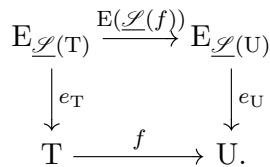
\includegraphics[keepaspectratio]{images/part001_16180f76.jpg}}
\end{enumerate}

This follows from I, p.~54, formula (2) for the first, and it is an immediate consequence of the definitions for the second. This implies that for every pair \((\mathcal{F},\mathcal{G})\) of sheaves on B and every pair (T,U) of étale B-spaces, the maps \(\varphi\mapsto\mathrm{E}(\varphi)\) and \(f\mapsto\underline{\mathcal{L}}(f)\) considered above are bijective.

These results make it possible to deduce a statement about étale B-spaces from a statement about sheaves on B, and conversely.

\subsection{Direct image and inverse image of a sheaf}

Let A and B be topological spaces and \(u: A \rightarrow B\) a continuous map.

Let \(\mathcal{F} = (\mathcal{F}(\mathrm{U}), f_{\mathrm{UV}})\) be a presheaf on A. We define a presheaf \(\mathcal{F}'\) on B as follows: for every open set U of B, set \(\mathcal{F}'(\mathrm{U}) = \mathcal{F}(u^{-1}(\mathrm{U}))\) and for every pair (U, V) of open sets of B such that U \(\subset\) V, set \(f_{\mathrm{UV}}' = f_{u^{-1}(\mathrm{U})u^{-1}(\mathrm{V})}\) . Then \((\mathcal{F}'(\mathrm{U}), f_{\mathrm{UV}}')\) is a presheaf on B. We denote it by \(u_{*}(\mathcal{F})\) and call it the direct image presheaf of the presheaf \(\mathcal{F}\) under the map u.

If \((\mathrm{U}_{i})_{i\in\mathrm{I}}\) is a family of open sets of B, we have \(u^{-1}(\bigcup_{i\in\mathrm{I}}\mathrm{U}_{i})=\bigcup_{i\in\mathrm{I}}u^{-1}(\mathrm{U}_{i})\) and \(u^{-1}(\bigcap_{i\in\mathrm{I}}\mathrm{U}_{i})=\bigcap_{i\in\mathrm{I}}u^{-1}(\mathrm{U}_{i})\) (E, II, p.~25, prop. 3 and 4). It follows immediately that if F has property \((\mathrm{F}_{1})\) (resp. \((\mathrm{F}_{2})\) ) of sheaves (I, p.~43), then so does \(u_{*}(\mathcal{F})\) . Consequently, the direct image of a sheaf is a sheaf.

Let \(\mathcal{F}_1\) and \(\mathcal{F}_2\) be presheaves on A and let \(\varphi\colon\mathcal{F}_1\to\mathcal{F}_2\) be a morphism of presheaves. There then exists a unique morphism of presheaves \(u_*\varphi\colon u_*\mathcal{F}_1\to u_*\mathcal{F}_2\) such that for every open set U of B, the map \((u_*\varphi)(U)\colon(u_*\mathcal{F}_1)(U)\to(u_*\mathcal{F}_2)(U)\) is the map \(\varphi(u^{-1}(U))\colon\mathcal{F}_{1}(u^{-1}(U))\to\mathcal{F}_{2}(u^{-1}(U)).\) If \(\mathcal{F}_{3}\) is a presheaf on A and if \(\psi\colon\mathcal{F}_{2}\to\mathcal{F}_{3}\) is a morphism of presheaves, we have \(u_{*}(\psi\circ\varphi)=u_{*}(\psi)\circ u_{*}(\varphi)\) .

Let C be a topological space and let \(v: B \to C\) be a continuous map. If \(\mathcal{F}\) is a presheaf on A, the presheaves \(v_{*}(u_{*}(\mathcal{F}))\) and \((v \circ u)_{*}(\mathcal{F})\) coincide. If \(\varphi: \mathcal{F}_{1} \to \mathcal{F}_{2}\) is a morphism of presheaves on A, we have the equality \(v_{*}(u_{*}(\varphi)) = (v \circ u)_{*}(\varphi)\) .

Example 1. --- Let B be a topological space, A a subspace of B, and \(\mathcal{F} = (\mathcal{F}(U), f_{\mathrm{UV}})\) a presheaf on A. Denote by \(i: A \to B\) the canonical injection. We then have \(i_*(\mathcal{F}) = (\mathcal{F}'(U), f_{\mathrm{UV}}')\) where for every open set U of B, \(\mathcal{F}'(U) = \mathcal{F}(U \cap A)\) , and for every pair (U, V) of open sets of B with \(U \subset V\) , \(f_{\mathrm{UV}}' = f_{(\mathrm{U} \cap A)(\mathrm{V} \cap A)}\) .

Now let \(\mathcal{G}\) be a presheaf on B. We define the inverse image of the presheaf \(\mathcal{G}\) under \(u\) , and denote by \(u^{*}(\mathcal{G})\) the sheaf \(\underline{\mathcal{C}}_{\mathrm{B}}(\mathrm{A};\mathrm{E}_{\mathcal{G}})\) on A of B-morphisms with values in the B-space \(\mathrm{E}_{\mathcal{G}}\) (I, p.~45, example 4). It is canonically isomorphic to the sheaf on A of sections of the A-étale space \(\mathrm{A} \times_{\mathrm{B}} \mathrm{E}_{\mathcal{G}}\) (I, p.~9, prop. 3). From this we deduce (I, p.~52, example 2) a canonical isomorphism \(\varphi\) of the étale space associated with \(u^{*}(\mathcal{G})\) onto the A-space \(\mathrm{A} \times_{\mathrm{B}} \mathrm{E}_{\mathcal{G}}\) . If moreover \(\mathcal{G}\) is a sheaf, then for every point \(a\) of A there is a canonical bijection \(\psi_{a}: u^{*}(\mathcal{G})_{a} \to \mathcal{G}_{u(a)}\) : for every open neighborhood U of \(a\) in A and every B-morphism \(f: \mathrm{U} \to \mathrm{E}_{\mathcal{G}}\) , we have

\[
\varphi ([ \mathrm{U}, f, a ]) = (a, f (a)), \quad \psi_ {a} ([ \mathrm{U}, f, a ]) = f (a).
\]

Let \(\mathcal{G}_1\) and \(\mathcal{G}_2\) be presheaves on B and \(\varphi\colon\mathcal{G}_1\to\mathcal{G}_2\) a morphism of presheaves. By base change of the morphism of B-étale spaces \(\mathrm{E}(\varphi)\colon\mathrm{E}_{\mathcal{G}_1}\to\mathrm{E}_{\mathcal{G}_2}\) we deduce a morphism of A-étale spaces \(\mathrm{A}\times_{\mathrm{B}}\mathrm{E}_{\mathcal{G}_1}\to\mathrm{A}\times_{\mathrm{B}}\mathrm{E}_{\mathcal{G}_2}\) , whence a morphism of sheaves on A, \(u^{*}(\varphi)\colon u^{*}(\mathcal{G}_{1})\to u^{*}(\mathcal{G}_{2})\) . Let \(\mathcal{G}_3\) be a presheaf on B and \(\psi\colon\mathcal{G}_2\to\mathcal{G}_3\) a morphism of presheaves. We then have the equality \(u^{*}(\psi\circ\varphi)=u^{*}(\psi)\circ u^{*}(\varphi)\) .

Let C be a topological space and let \(v\colon B \to C\) be a continuous map. If \(\mathcal{G}\) is a presheaf on C, the sheaves \(u^{*}(v^{*}(\mathcal{G}))\) and \((v \circ u)^{*}(\mathcal{G})\) are canonically identified (I, p.~5). If \(\varphi\colon\mathcal{G}_{1} \to \mathcal{G}_{2}\) is a morphism of presheaves on C, we moreover have \(u^{*}(v^{*}(\varphi)) = (v \circ u)^{*}(\varphi)\) .

Remark. --- The canonical morphism \(\sigma_{\mathcal{G}}\colon\mathcal{G}\to\widetilde{\mathcal{G}}\) of I, p.~53 corresponds in terms of étale spaces to the isomorphism \(j_{\mathcal{G}}\) of Proposition 2 of I, p.~53. It follows that \(u^{*}(\sigma_{\mathcal{G}})\) is an isomorphism. In particular, if \(A = B\) and \(u = \mathrm{Id}_A\) , the presheaf \(u^{*}(\mathcal{F})\) is the sheaf \(\widetilde{\mathcal{F}}\) .

Example 2. --- Let B be a topological space and A a subspace of B. Denote by \(i\colon\mathrm{A}\to\mathrm{B}\) the canonical injection. For every sheaf \(\mathcal{G}\) on B, denote by \(\mathcal{G}_{\mathrm{A}}\) the sheaf \(i^{*}(\mathcal{G})\) and call \(\mathcal{G}_{\mathrm{A}}\) the sheaf on A induced by the sheaf \(\mathcal{G}\) . The sheaf \(\mathcal{G}_{\mathrm{A}}\) is identified with the sheaf \(\underline{\mathcal{L}}(\mathrm{A};(\mathrm{E}_{\mathcal{G}})_{\mathrm{A}})\) of sections of the A-étale space induced by \(\mathrm{E}_{\mathcal{G}}\) over A.

Suppose that A is an open subspace of B, and let \(\mathcal{G}\) be a sheaf on B. By definition, the sheaf \(\mathcal{G}_{\mathrm{A}}\) is the sheaf \(\widetilde{\mathcal{G}}\mid \mathrm{A}\) deduced from \(\widetilde{\mathcal{G}}\) by restriction to the open set A (I, p.~43). Let \(\sigma_{\mathcal{G}}\colon \mathcal{G}\to \widetilde{\mathcal{G}}\) be the canonical isomorphism (I, p.~55, cor. 1). Then \(\sigma_{\mathcal{G}}\mid \mathrm{A}\) is a canonical isomorphism from the sheaf \(\mathcal{G}\mid \mathrm{A}\) onto the sheaf \(\mathcal{G}_{\mathrm{A}}\), called the canonical isomorphism of \(\mathcal{G}\mid \mathrm{A}\) onto \(\mathcal{G}_{\mathrm{A}}\) .

\subsection{\texorpdfstring{The homomorphisms \(\alpha\) and \(\beta\) ; adjunction}{The homomorphisms alpha and beta ; adjunction}}

Let A and B be topological spaces and let \(u\colon\mathrm{A}\to\mathrm{B}\) be a continuous map. Let \(\mathcal{G}\) be a presheaf on B. By definition of the direct image of presheaves, a section of the sheaf \(u_{*}u^{*}\mathcal{G}\) over an open set U of B is a section of the sheaf \(u^{*}\mathcal{G}\) over the open set \(u^{-1}(\mathrm{U})\) of A, that is, a B-morphism \(u^{-1}(\mathrm{U})\to\mathrm{E}_{\mathcal{G}}\) . One thus defines a morphism of sheaves \(\widetilde{\mathcal{G}}\to u_{*}u^{*}\mathcal{G}\) by associating to the section \(s\) of \(\mathrm{E}_{\mathcal{G}}\) over an open set U of B the section \(s\circ u\) of \(\mathrm{E}_{\mathcal{G}}\) over \(u^{-1}(\mathrm{U})\) . The composition of this morphism and the canonical morphism \(\sigma_{\mathcal{G}}\colon\mathcal{G}\to\widetilde{\mathcal{G}}\) (I, p.~53) is a morphism of presheaves \(\mathcal{G}\to u_{*}u^{*}\mathcal{G}\) which will be denoted by \(\beta_{\mathcal{G}}^{u}\) , or even \(\beta_{\mathcal{G}}\) if there is no ambiguity about the map \(u\) .

Remarks. --- 1) Let A, B, C be topological spaces, let \(u\colon A \to B\) , \(v\colon B \to C\) be continuous maps; set \(w = v \circ u\) . Let \(\mathcal{G}\) be a presheaf on C.

Let U be an open set of C and let s be a section of \(E_{G}\) over U. Then \(\beta_{\mathcal{G}}^{v}(s)\) is the section \(s \circ v\) of \(E_{G}\) over \(v^{-1}(U)\) , and \(v_{*}(\beta_{v^{*}\mathcal{G}}^{u})(\beta_{\mathcal{G}}^{v}(s))\) is the section \(s \circ v \circ u = s \circ w\) of \(E_{G}\) over \(u^{-1}(v^{-1}(U)) = w^{-1}(U)\) .

It follows that \(\beta_{\mathcal{G}}^{w} = v_{*}(\beta_{v^{*}\mathcal{G}}^{u})\circ \beta_{\mathcal{G}}^{v}\) .

\begin{enumerate}
\def\labelenumi{\arabic{enumi})}
\setcounter{enumi}{1}
\tightlist
\item
  If \(\gamma\colon\mathcal{G}_{1}\to\mathcal{G}_{2}\) is a morphism of presheaves on B, the morphisms of presheaves \(\beta_{\mathcal{G}_{2}}\circ\gamma\) and \(u_{*}u^{*}(\gamma)\circ\beta_{\mathcal{G}_{1}}\) are equal. Indeed, if V is an open set of B and \(s\in\mathcal{G}_{1}(V)\) , \(\beta_{\mathcal{G}_{1}}(s)\) is the section \(t\) of A \(\times_{B}E_{\mathcal{G}_{1}}\) over \(u^{-1}(V)\) , defined by \(x\mapsto(x,[V,s,u(x)])\) . The image of \(t\) under \(u^{*}(\gamma)\) is thus the section of A \(\times_{B}E_{\mathcal{G}_{2}}\) over \(u^{-1}(V)\) given by \(x\mapsto(x,[V,\gamma(s),u(x)])\) . It follows that \(u_{*}u^{*}(\gamma)\circ\beta_{\mathcal{G}_{1}}(s)=\beta_{\mathcal{G}_{2}}(\gamma(s))\) .
\end{enumerate}

PROPOSITION 4. --- Let A and B be topological spaces, let \(u\colon A\to B\) be a continuous map, let \(\mathcal{G}\) be a presheaf on B, and let \(\mathcal{F}\) be a sheaf on A.

For every morphism of presheaves \(\varphi\colon\mathcal{G}\to u_{*}\mathcal{F}\) , there exists a unique morphism of sheaves \(\psi\colon u^{*}(\mathcal{G})\to\mathcal{F}\) such that \(\varphi=u_{*}(\psi)\circ\beta_{\mathcal{G}}\) .

In other words, the canonical map

\[
\operatorname{Mor} \left(u ^ {*} (\mathcal {G}), \mathcal {F}\right)\rightarrow \operatorname{Mor} \left(\mathcal {G}, u _ {*} (\mathcal {F})\right), \quad \psi \mapsto u _ {*} (\psi) \circ \beta_ {\mathcal {G}}
\]

is a bijection.

Using the notation of Proposition 4, we will sometimes denote \(\psi = \varphi^{\sharp}\) and \(\varphi = \psi^{\flat}\) .

Let us prove Proposition 4. By Remark 2 applied to the morphism \(\sigma_{\mathcal{G}}: \mathcal{G} \to \widetilde{\mathcal{G}}\) , the morphism \(\beta_{\mathcal{G}}\) is equal to the composition

\[
u _ {*} (u ^ {*} (\sigma_ {\mathcal {G}}) ^ {- 1}) \circ \beta_ {\widetilde {\mathcal {G}}} \circ \sigma_ {\mathcal {G}},
\]

where \(u^{*}(\sigma_{\mathcal{G}}) \colon u^{*}(\mathcal{G}) \to u^{*}(\widetilde{\mathcal{G}})\) is the canonical isomorphism of Remark I, p.~58. Let \(\widetilde{\varphi} \colon \widetilde{\mathcal{G}} \to u_{*}\mathcal{F}\) be the unique morphism of sheaves such that \(\widetilde{\varphi} \circ \sigma_{\mathcal{G}} = \varphi\) (I, p.~54, prop. 3). It then suffices to show that there exists a unique morphism of sheaves \(\widetilde{\psi} \colon u^{*}(\mathcal{G}) \to \mathcal{F}\) such that \(u_{*}(\widetilde{\psi}) \circ \beta_{\widetilde{\mathcal{G}}} = \widetilde{\varphi}\) .

We may therefore assume that \(\mathcal{G}\) is a sheaf. For a morphism of sheaves \(\psi: u^{*}(\mathcal{G}) \to \mathcal{F}\) to satisfy the conclusion of Proposition 4, it is necessary and sufficient that for every open set V of B and every section \(t\) of \(\mathrm{E}_{\mathcal{G}}\) above V, one has

\[
\varphi_{\mathrm{V}}(t) = \psi_{u^{-1}(\mathrm{V})}(t \circ u \mid u^{-1}(\mathrm{V})).\tag{6}
\]

Let \(U_{0}\) be an open subset of A and \(s_{0}\) be an element of \(u^{*}(\mathcal{G})(\mathrm{U}_{0})\), in other words, a B-morphism from \(U_{0}\) into \(E_{\mathcal{G}}\) . Let \(\mathrm{S}(\mathrm{U}_{0}, s_{0})\) be the set of triples \((\mathrm{U}, \mathrm{V}, t)\) where U is an open subset of A contained in \(U_{0}\) , V is an open subset of B such that \(u(\mathrm{U}) \subset \mathrm{V}\), and let t be a section of \(E_{\mathcal{G}}\) above V such that one has

\[
t \circ u \mid \mathrm{U} = s _ {0} \mid \mathrm{U}.\tag{7}
\]

If \(U_{1}\) and \(U_{2}\) are open subsets of A with \(U_{1} \subset U_{2}\) , denote by \(f_{U_{1}U_{2}}\) the restriction map \(\mathcal{F}(U_{2}) \to \mathcal{F}(U_{1})\) . For every \((\mathrm{U}, \mathrm{V}, t) \in \mathrm{S}(\mathrm{U}_{0}, s_{0})\) we then have the relation

\[
\begin{array}{l} f_{\mathrm{U}\mathrm{U}_{0}}(\psi_{\mathrm{U}_{0}}(s_{0})) = \psi_{\mathrm{U}}(s_{0} \mid \mathrm{U}) \\ \qquad = \psi_{\mathrm{U}}(t \circ u \mid \mathrm{U}) \\ \qquad = f_{\mathrm{U}u^{-1}(\mathrm{V})}(\psi_{u^{-1}(\mathrm{V})}(t \circ u \mid u^{-1}(\mathrm{V}))). \end{array}
\]

Consequently, if \(\psi \colon u^{*}(\mathcal{G})\to \mathcal{F}\) satisfies (6), we have

\[
f_{\mathrm{U}\mathrm{U}_{0}}(\psi_{\mathrm{U}_{0}}(s_{0})) = f_{\mathrm{U}u^{-1}(\mathrm{V})}(\varphi_{\mathrm{V}}(t)).\tag{8}
\]

Let us prove that, for every point \(a\) of \(\mathrm{U}_0\) , there exists a triple \((\mathrm{U},\mathrm{V},t)\in \mathrm{S}(\mathrm{U}_0,s_0)\) such that \(a\in \mathrm{U}\). Indeed, let \(a\) be a point of \(\mathrm{U}_0\). There exists an open neighborhood V in B containing \(u(a)\) and a section \(t\) of the étale space \(\mathbf{E}_{\mathcal{G}}\) over V such that \(t(u(a)) = s_0(a)\) (I, p.~33, prop. 9). Let \(\mathrm{U}_1 = u^{-1} (\mathrm{V})\cap \mathrm{U}_0\) . The sections \(s_0\mid \mathrm{U}_1\) and \(t\circ u\mid \mathrm{U}_1\) of the étale space over \(\mathrm{U}_1\), \(\mathbf{E}_{\mathcal{G}}\times_{\mathrm{B}}\mathrm{U}_1\), coincide at the point \(a\). By Proposition 11, b) of I, p.~34, the set of points where they coincide is an open set U of \(\mathrm{U}_1\) which contains \(a\). The triple \((\mathrm{U},\mathrm{V},t)\) then belongs to \(\mathrm{S}(\mathrm{U}_0,s_0)\) .

Formula (8) and the property \((\mathrm{F}_{1})\) of sheaves (I, p.~43) then imply the uniqueness of \(\psi\) .

Let (U, V, t) and \((\mathrm{U}^{\prime}, \mathrm{V}^{\prime}, t^{\prime})\) be elements of \(\mathrm{S}(\mathrm{U}_{0}, s_{0})\) . By relation (7), the restrictions of t and \(t^{\prime}\) to \(u(\mathrm{U} \cap \mathrm{U}^{\prime})\) coincide. By prop. 11, b) of I, p.~34, there exists an open set W of B such that \(u(\mathrm{U} \cap \mathrm{U}^{\prime}) \subset \mathrm{W} \subset \mathrm{V} \cap \mathrm{V}^{\prime}\) and that \(t \mid W = t^{\prime} \mid W\) . We therefore have

\[
f_{u^{-1}(\mathrm{W})u^{-1}(\mathrm{V})}(\varphi_{\mathrm{V}}(t)) = \varphi_{\mathrm{W}}(t\mid \mathrm{W}) = \varphi_{\mathrm{W}}(t^{\prime}\mid \mathrm{W}) = f_{u^{-1}(\mathrm{W})u^{-1}(\mathrm{V}^{\prime})}(\varphi_{\mathrm{V}^{\prime}}(t^{\prime}))
\]

whence

\[
f_{(\mathrm{U}\cap\mathrm{U}^{\prime})u^{-1}(\mathrm{V})}(\varphi_{\mathrm{V}}(t)) = f_{(\mathrm{U}\cap\mathrm{U}^{\prime})u^{-1}(\mathrm{V}^{\prime})}(\varphi_{\mathrm{V}^{\prime}}(t^{\prime})).\tag{9}
\]

By the properties \((\mathrm{F}_{1})\) and \((\mathrm{F}_{2})\) for the sheaf F, there exists a unique element \(s'\) of \(\mathcal{F}(\mathrm{U}_{0})\) such that for every triple \((\mathrm{U},\mathrm{V},t)\) of

\(\mathrm{S}(\mathrm{U}_{0},s_{0})\) one has:

\[
f_{\mathrm{U}\mathrm{U}_{0}}(s^{\prime}) = f_{\mathrm{U}u^{-1}(\mathrm{V})}(\varphi_{\mathrm{V}}(t)).\tag{10}
\]

Denote by \(\psi_{\mathrm{U}_{0}}(s_{0})\) this element.

Let \(U_{1}\) be an open set contained in \(U_{0}\) and let \(s_{1}=s_{0}|U_{1}\) . If \((\mathrm{U},\mathrm{V},t)\in\mathrm{S}(\mathrm{U}_{1},s_{1})\) , then U is an open set contained in \(U_{0}\) and \(t\circ u|U=s_{1}|U=s_{0}|U\) , therefore \((\mathrm{U},\mathrm{V},t)\in\mathrm{S}(\mathrm{U}_{0},s_{0})\) , and relation (10) then implies that

\[
f_{\mathrm{U}\mathrm{U}_{1}}(f_{\mathrm{U}_{1}\mathrm{U}_{0}}(\psi_{\mathrm{U}_{0}}(s_{0}))) = f_{\mathrm{U}\mathrm{U}_{0}}(\psi_{\mathrm{U}_{0}}(s_{0})) = f_{\mathrm{U}u^{-1}(\mathrm{V})}(\varphi_{\mathrm{V}}(t)).
\]

By definition of \(\psi_{\mathrm{U}_{1}}(s_{1})\) , we therefore have \(\psi_{\mathrm{U}_{1}}(s_{1}) = f_{\mathrm{U}_{1}\mathrm{U}_{0}}(\psi_{\mathrm{U}_{0}}(s_{0}))\) . This proves that the family \(\psi = (\psi_{\mathrm{U}})\) is a morphism of sheaves from \(u^{*}(\mathcal{G})\) into \(\mathcal{F}\).

Let us prove that \(\psi\) satisfies relation (6). Let V be an open subset of B and \(t\) be a section of \(\mathrm{E}_{\mathcal{G}}\) above V. If \(\mathrm{U} = u^{-1}(\mathrm{V})\) and if \(s = t \circ u \mid \mathrm{U}\) , the triple \((\mathrm{U}, \mathrm{V}, t)\) belongs to \(\mathrm{S}(\mathrm{U}, s)\) and relation (6) is an immediate consequence of relation (10), applied to \(\mathrm{U} = \mathrm{U}_0\) .

PROPOSITION 5. — Let A and B be topological spaces and let u: A → B be a continuous map.

\begin{enumerate}
\def\labelenumi{\alph{enumi})}
\tightlist
\item
  Let \(\mathcal{G}_1\) and \(\mathcal{G}_2\) be presheaves on B and let \(\gamma\colon\mathcal{G}_1\to\mathcal{G}_2\) be a morphism of presheaves. Let also \(\mathcal{F}\) be a sheaf on A and \(\varphi\colon\mathcal{G}_2\to u_*\mathcal{F}\) a morphism of presheaves. We have the equality
\end{enumerate}

\[
(\varphi \circ \gamma) ^ {\sharp} = \varphi^ {\sharp} \circ u ^ {*} (\gamma).\tag{11}
\]

\begin{enumerate}
\def\labelenumi{\alph{enumi})}
\setcounter{enumi}{1}
\tightlist
\item
  Let \(\mathcal{F}_1\) and \(\mathcal{F}_2\) be sheaves on A and let \(\mathcal{G}\) be a presheaf on B. Let \(\varphi\colon\mathcal{F}_1\to\mathcal{F}_2\) be a morphism of sheaves and let \(\gamma\colon\mathcal{G}\to u_*\mathcal{F}_1\) be a morphism of presheaves. We have the relation
\end{enumerate}

\[
(u _ {*} (\varphi) \circ \gamma) ^ {\sharp} = \varphi \circ \gamma^ {\sharp}.
\]

\begin{enumerate}
\def\labelenumi{\alph{enumi})}
\tightlist
\item
  By definition of \(\varphi^{\sharp}\) and Remark 2 of I, p.~60, we have
\end{enumerate}

\[
\varphi \circ \gamma = u _ {*} (\varphi^ {\sharp}) \circ \beta_ {\mathcal {G} _ {2}} \circ \gamma = u _ {*} (\varphi^ {\sharp}) \circ u _ {*} u ^ {*} (\gamma) \circ \beta_ {\mathcal {G} _ {1}}.
\]

Therefore, \(\varphi \circ \gamma = u_{*}(\varphi^{\sharp}\circ u^{*}(\gamma))\circ \beta_{\mathcal{G}_{1}}\); whence relation (11).

\begin{enumerate}
\def\labelenumi{\alph{enumi})}
\setcounter{enumi}{1}
\tightlist
\item
  By definition of \(\gamma^{\sharp}\) , we have
\end{enumerate}

\[
u _ {*} (\varphi) \circ \gamma = u _ {*} (\varphi) \circ u _ {*} (\gamma^ {\sharp}) \circ \beta_ {\mathcal {G}} = u _ {*} (\varphi \circ \gamma^ {\sharp}) \circ \beta_ {\mathcal {G}},
\]

whence the announced relation, taking into account the definition of \((u_{*}(\varphi)\circ\gamma)^{\sharp}\) .

Set \(\alpha_{\mathcal{F}} = \mathrm{Id}_{u_*(\mathcal{F})}^\sharp\) ; it is the unique morphism of sheaves \(\rho \colon u^*(u_*(\mathcal{F})) \to \mathcal{F}\) such that

\[
\operatorname{Id} _ {u _ {*} (\mathcal {F})} = u _ {*} (\rho) \circ \beta_ {u _ {*} (\mathcal {F})}.
\]

Relation (11) applied to \(\mathcal{G}_2 = u_*(\mathcal{F})\) and to the morphism \(\varphi = \mathrm{Id}_{u_*(\mathcal{F})}\) yields, for every morphism of presheaves \(\gamma\colon\mathcal{G}\to u_*(\mathcal{F})\), the factorization

\[
\gamma^ {\sharp} = \alpha_ {\mathcal {F}} \circ u ^ {*} (\gamma).
\]

It then follows from Proposition 4 that for every morphism of sheaves \(\psi\) from \(u^{*}(\mathcal{G})\) into \(\mathcal{F}\) , \(\psi^{\flat}\) is the unique morphism \(\varphi\colon\mathcal{G}\to u_{*}(\mathcal{F})\) such that \(\psi=\alpha_{\mathcal{F}}\circ u^{*}(\varphi)\) .

Examples. --- 1) Consider a topological space B, a subspace A of B, and denote by \(i\colon A \to B\) the canonical injection. Let \((E,p)\) and \((E',p')\) be B-spaces. Take for \(\mathcal{G}\) the sheaf \(\underline{\mathcal{M}or}_{B}(E;E')\) (I, p.~45, Example 4) and for \(\mathcal{F}\) the sheaf \(\underline{\mathcal{M}or}_{A}(E_{A};E_{A}')\) . For every open set V of B and every V-morphism \(f\colon E_{V} \to E_{V}'\) , set \(\varphi_{V}(f) = f_{V \cap A}\) , where \(f_{V \cap A}\) is the \((V \cap A)\) -morphism from \(E_{V \cap A}\) into \(E_{V \cap A}'\) induced by \(f\) . The family \(\varphi = (\varphi_{V})\) thus defined is a morphism of sheaves from \(\mathcal{G}\) into \(i_*\mathcal{F}\) . By Proposition 4, there exists a unique morphism of sheaves \(\psi\colon \underline{\mathcal{M}or}_{B}(E;E')_{A} \to \underline{\mathcal{M}or}_{A}(E_{A};E_{A}')\) such that one has

\[
\psi_ {\mathrm{V} \cap \mathrm{A}} (\sigma_ {\mathcal {G}} (\mathrm{V}, f) \mid \mathrm{V} \cap \mathrm{A}) = f _ {\mathrm{V} \cap \mathrm{A}}\tag{12}
\]

for every open set V of B and every \(f \in \mathcal{C}_{\mathrm{V}}(\mathrm{E}_{\mathrm{V}}; \mathrm{E}_{\mathrm{V}}^{\prime})\) . The morphism \(\psi\) is called the canonical morphism from \(\underline{\mathcal{M}or_{B}}(\mathrm{E}; \mathrm{E}^{\prime})_{\mathrm{A}}\) into \(\underline{\mathcal{M}or_{A}}(\mathrm{E}_{\mathrm{A}}; \mathrm{E}_{\mathrm{A}}^{\prime})\) .

If A is reduced to a single point \(a\) , this morphism is identified with the morphism from the stalk at \(a\) of the sheaf \(\underline{\mathcal{M}or}_{\mathrm{B}}(\mathrm{E};\mathrm{E}^{\prime})\) into the set \(\mathcal{C}(\mathrm{E}_a;\mathrm{E}_a')\) .

By passing to subsheaves, the morphism \(\psi\) induces a canonical morphism of \(\mathcal{I}som_{\mathrm{B}}(\mathrm{E};\mathrm{E}')_{\mathrm{A}}\) into \(\mathcal{I}som_{\mathrm{A}}(\mathrm{E}_{\mathrm{A}};\mathrm{E}_{\mathrm{A}}^{\prime})\) .

\begin{enumerate}
\def\labelenumi{\arabic{enumi})}
\setcounter{enumi}{1}
\tightlist
\item
  Let A, B, C be topological spaces and let \(u\colon A\to B\) , \(v\colon B\to C\) be continuous maps; set \(w=v\circ u\) . Let E and E' be C-spaces. The canonical morphism of \(\underline{\mathcal{M}or}_{C}(E;E')_{A}\) into \(\underline{\mathcal{M}or}_{A}(E_{A};E'_{A})\) is the composite of the morphism \(\underline{\mathcal{M}or}_{C}(E;E')_{A}\to\underline{\mathcal{M}or}_{B}(E_{B};E'_{B})_{A}\) deduced from the canonical morphism of \(\underline{\mathcal{M}or}_{C}(E;E')_{B}\) into \(\underline{\mathcal{M}or}_{B}(E_{B};E'_{B})\) and the canonical morphism of \(\underline{\mathcal{M}or}_{B}(E_{B},E'_{B})_{A}\) into \(\underline{\mathcal{M}or}_{A}(E_{A},E'_{A})\) .
\end{enumerate}
